% Class def
\documentclass[xcolor=table,serif]{beamer} 
%\usepackage{pgfpages}
%\pgfpagesuselayout{8 on 1}[a4paper,border shrink=5mm]
% %Language and accents
\usepackage[spanish]{babel}
\usepackage[utf8]{inputenc}
% For text justification
\usepackage{ragged2e}
\usepackage{animate} %need the animate.sty file 
% ams math packages
\usepackage{amsmath}
\usepackage{amsfonts}
\usepackage{amssymb}
% % Images 
 \usepackage{graphicx}
 \usepackage{subfigure}
 \usepackage[labelformat=empty]{caption}
 \setbeamerfont{caption}{size=\scriptsize}
% theme 
\usetheme[]{Madrid}
%\usepackage{colortbl}
%\usepackage[table]{xcolor} 
\usepackage{subfigure}
%\usetheme{Boadilla} 
%\usecolortheme{dolphin} 
\graphicspath{{img/}}
% Links and hyperlinks
 \usepackage{url}
% \usepackage{hyperref}
 \hypersetup{colorlinks, linkcolor = blue, urlcolor = blue}
% Default fixed font does not support bold face
\DeclareFixedFont{\ttb}{T1}{txtt}{bx}{n}{8} % for bold
\DeclareFixedFont{\ttm}{T1}{txtt}{m}{n}{8}  % for normal
% For text boxes
\usepackage{fancybox}
% Custom colors
\usepackage{color}
\definecolor{deepblue}{rgb}{0,0,0.5}
\definecolor{deepred}{rgb}{0.6,0,0}
\definecolor{deepgreen}{rgb}{0,0.5,0}

\usepackage{listings}
% Python style for highlighting
\newcommand\pythonstyle{\lstset{
language=Python,
basicstyle=\ttm,
otherkeywords={self},             % Add keywords here
keywordstyle=\ttb\color{deepblue},
emph={MyClass,__init__},          % Custom highlighting
emphstyle=\ttb\color{deepred},    % Custom highlighting style
stringstyle=\color{deepgreen},
frame=tb,                         % Any extra options here
showstringspaces=false            % 
}}
% Python environment

\lstnewenvironment{python}[1][]
{
\pythonstyle
\lstset{#1}
}
{}

\date{\today} 
\logo{Ingeniería Física
\includegraphics[width=1cm]{eafit_escudo}} 
\author[]{Santiago Echeverri Chac\'on\\ Asesor: \\ Nicol\'as Guar\'in Zapata}
\title[Trabajo de grado]{Una plataforma para la simulación de propagación de luz en estructuras fotónicas cristalinas con defectos.}
\subtitle{Trabajo de grado}
\institute{Universidad EAFIT}

\begin{document}

\begin{frame}
\titlepage
\end{frame}
\frame{
\footnotesize 
\frametitle{Contenido}
\tableofcontents
}
\AtBeginSection[]
		{
			 \begin{frame}
			  \frametitle{Contenido}
			  \footnotesize 
			\tableofcontents[currentsection]%,hideothersubsections]
			  \normalsize
 			\end{frame}
		}
		
\section{Introducción}
		
	\subsection{Planteamiento del Problema}
	\begin{frame}
	\frametitle{Planteamiento del problema}
	\justifying
	En el trabajo que se presenta aquí se propuso construir un paquete de herramientas de software que permitiera el análisis de propagación de campos electromagnéticos en el contexto de cristales fotónicos (PCs), con la capacidad de modelar defectos.  \\
	Esta presentación se propone responder las siguientes preguntas:
	\vskip20pt
	\begin{columns}[t]
		\column{0.2 \textwidth}
				\shadowbox{¿Por qué?}
		\column{0.2 \textwidth}
				\shadowbox{¿Para qué?}
		\column{0.2 \textwidth}
				\shadowbox{¿Cómo?}
		\column{0.2 \textwidth}
				\shadowbox{¿Qué?}
	\end{columns}

	\end{frame}
	\begin{frame}
	\frametitle{Objetivos planteados en el anteproyecto}
		\begin{block}{Objetivos Generales}
		\begin{itemize}
			\item Construir una plataforma de software capaz de simular propagación de campos electromagnéticos en PCs con defectos tales como cavidades e inclusiones.
			\item La arquitectura de la plataforma debe ser diseñada de tal forma que se faciliten: 
			\begin{itemize}
				\item las futuras actualizaciones,
				\item soporte de esquemas de optimización,
				\item e integración con otros tipos de simulaciones como aquellas de confinamiento de electrones en pozos de potencial y cristales. 	
			\end{itemize}
		\end{itemize}
		\end{block}
		\end{frame}
		\begin{frame}
		\begin{block}{Objetivos Espec\'ificos}
	    \begin{enumerate}
			\item Adquirir la teoría, particularmente:
			% Adquirir la teoría detrás de los campos electromagnéticos y sus aplicaciones en el contexto de cristales fotónicos. Particularmente: 
			\begin{enumerate}
				\item Electromagnetismo y modelación de cristales fotónicos, 
	 			\item Así como, métodos computacionales en  electromagnetismo.
	 		\end{enumerate}
			\item Definir requerimientos de implementación. 
			\item Programar algoritmos para:
				\begin{enumerate}
					\item Problemas escalares simples en 2D.	
					\item Problemas vectoriales, estacionarios con condiciones no periódicas.
					\item Soluciones vectoriales para problemas dependientes del tiempo.
					\item Introducir condiciones de periodicidad.
				\end{enumerate}
			\item Documentar los resultados.
		\end{enumerate}
		\end{block}
	\end{frame}
	\subsection{Justificación}
	\begin{frame}
	\frametitle{Justificación}
	De una forma u otra el mundo que hemos creado es una consecuencia de nuestra habilidad para entender y transformar materiales.
	\note{Nuestro hábitat artificial como consecuencia de la capacidad para entender las propiedades de los materiales.}
	\note{Proceso empíricos, y la presión de la supervivencia del más apto, llevaron a la humanidad a desarrollar nuevos materiales con los cuales construir, entro otras cosas, armas y armaduras.}	
	\vskip10pt
	\begin{columns}
	
	\column{0.25 \textwidth}
	\centerline{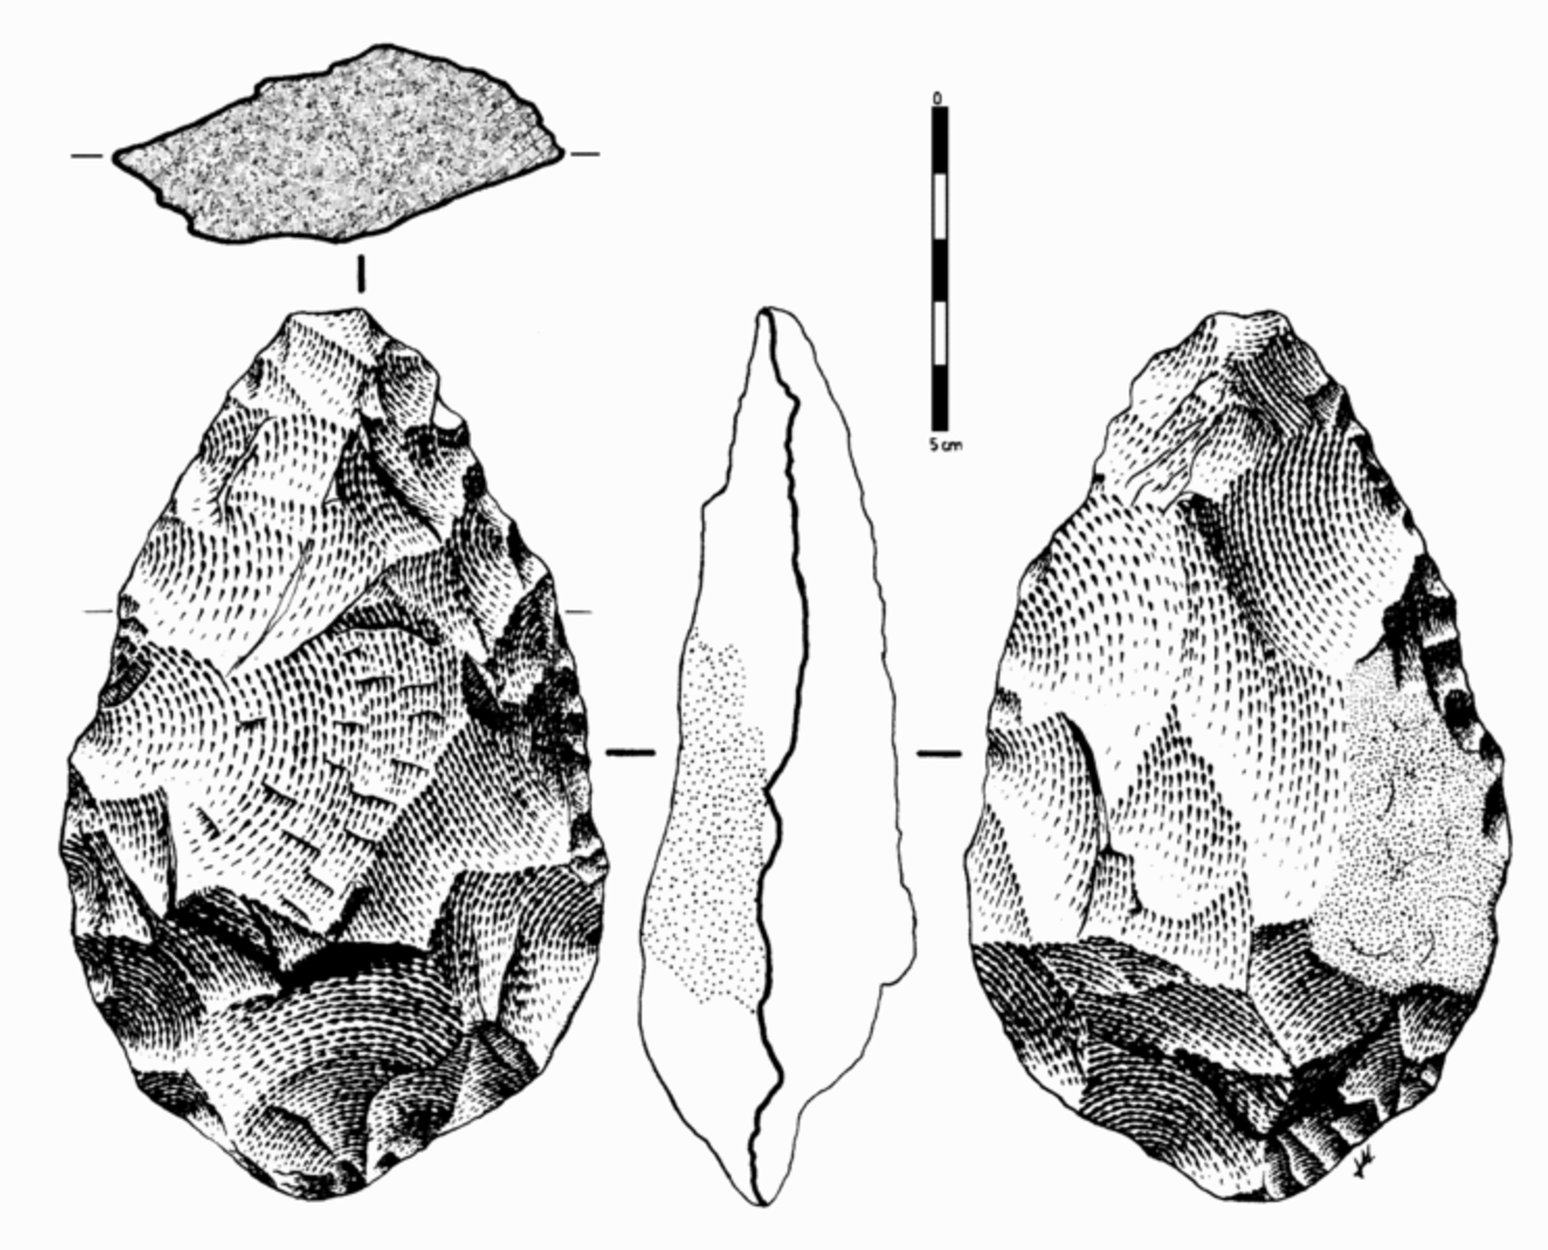
\includegraphics[scale=0.1]{stone_tool.pdf}}

	\column{0.25 \textwidth}
	\centerline{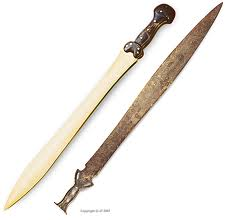
\includegraphics[scale=0.25]{bronze_sword.jpeg}}

	\column{0.25 \textwidth}
	\centerline{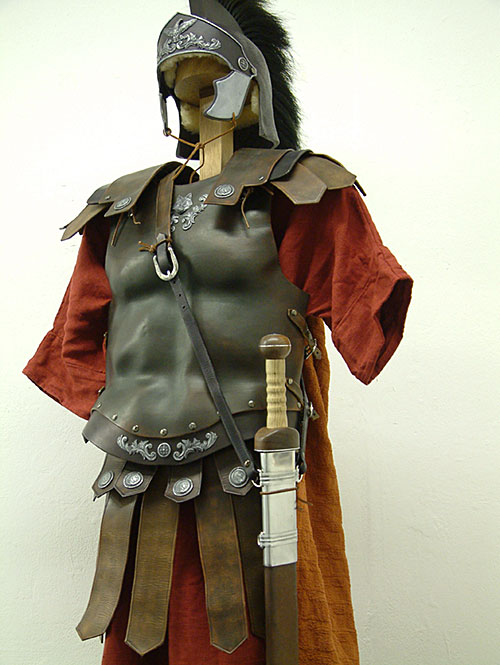
\includegraphics[scale=0.09]{roman_armour.jpg}}

	\column{0.25 \textwidth}
	\centerline{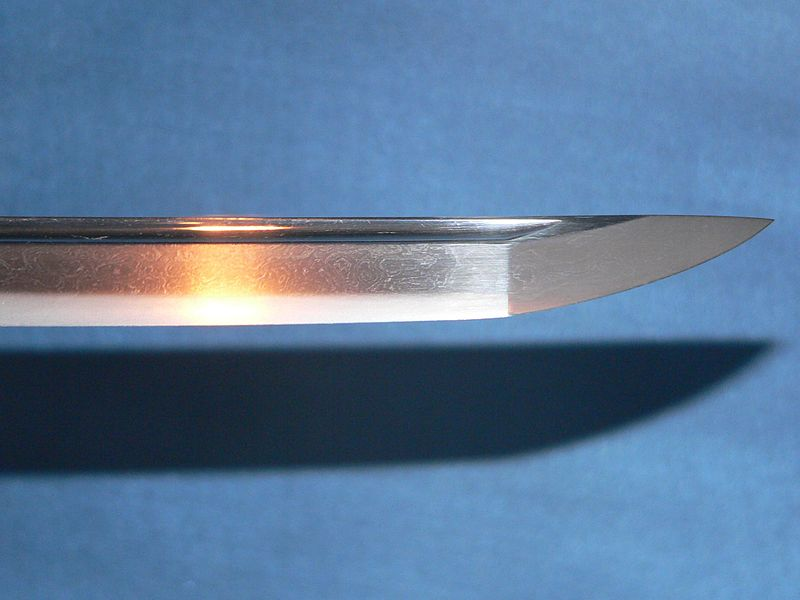
\includegraphics[scale=0.08]{katana.jpg}}
	\note{La katana como uno de los pináculos de el proceso empírico de formación de aleaciones y combinación de propiedades en materiales para obtener un resultado específico}
	\end{columns}
	\vskip10pt
	\pause
	\begin{columns}
	\column{0.25 \textwidth}
	\centerline{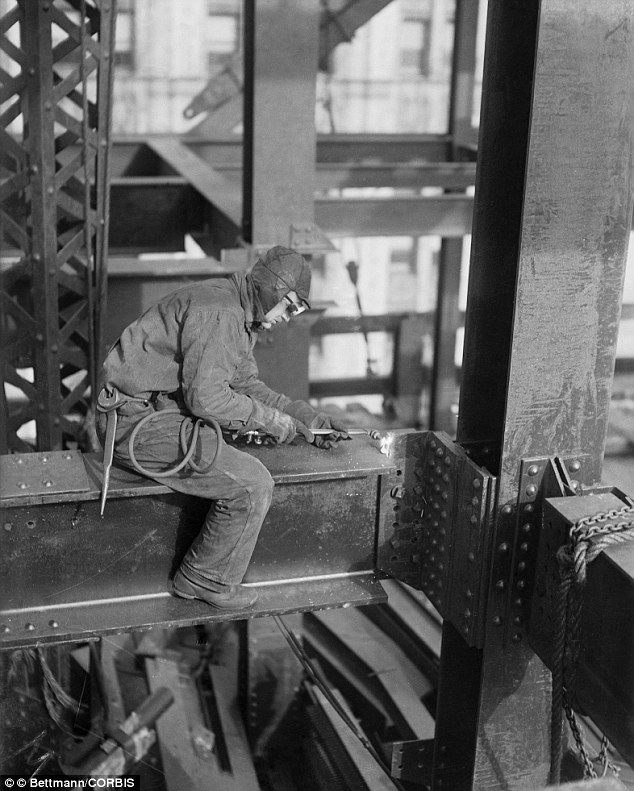
\includegraphics[scale=0.1]{skyscrapper.jpg}}

	\column{0.2 \textwidth}
	\centerline{
\includegraphics[scale=0.05]{plastic.jpg}}

	\column{0.25 \textwidth}
	\centerline{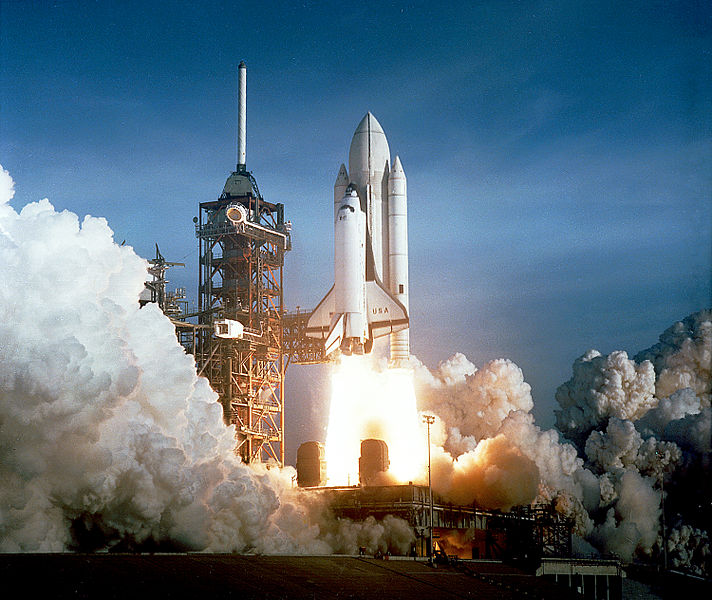
\includegraphics[scale=0.5]{space_age.jpg}}	

	\column{0.25 \textwidth}
	\centerline{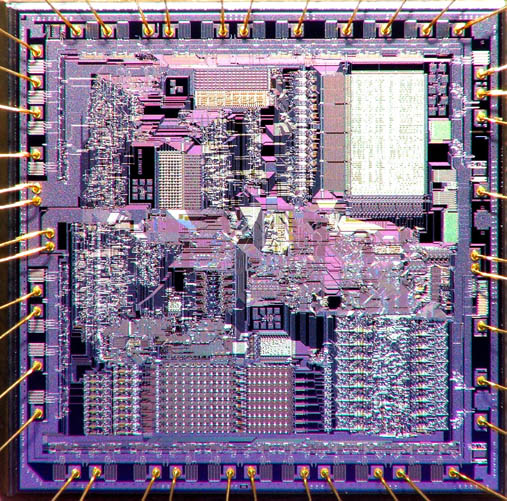
\includegraphics[scale=0.1]{microprocessor.jpg}}	
	\end{columns}
	\end{frame}
	
	\begin{frame}
	En particular, el entendimiento de las propiedades de los materiales semiconductores nos permitió diseñar materiales capaces de  conducir electricidad de manera condicionada. Esto fue la semilla de un cambio de paradigma que dio comienzo a la era de la información.
	\vskip20pt
	\begin{columns}
	\begin{column}{0.2 \textwidth}
	\centering
	\begin{figure}
	\includegraphics<1>[scale=0.2]{Transistor.pdf}
	\only<1>{\caption{Primer transistor 1947}	}
	\includegraphics<2>[scale=0.2]{early_microprocessor.jpg}
	\only<2>{\caption{Microprocesador AL1 (1969)} }
	\end{figure}
	\end{column}
\note{http://www.tayloredge.com/museum/processor/processorhistory.html}
	\begin{column}{0.2 \textwidth}
	\centering
	\begin{figure}
	\includegraphics<1>[scale=0.25]{transistors.pdf}
	\only<1>{\caption{Micrografía de un transistor FET (2009)  \href{http://infoscience.epfl.ch/record/141935}{\cite{A.M.Apetrei2005}}}}
	\note{Transistor de efecto campo}
	\includegraphics<2>[scale=0.2]{2000_Pentium4.jpg}
	\only<2>{\caption{Intel pentium 4 (2000)}}
	\end{figure}	
	\end{column}
	\end{columns}	
	\end{frame}			\note{http://www.sciencedaily.com/releases/2010/04/100428110806.htm}
	
	\frame{
	\frametitle{Justificación}
	De usar y transformar pasamos a entender, ahora empezamos a diseñar materiales con propiedades nuevas. Este es el campo de los meta-materiales.
		\begin{columns}[t]
			\begin{column}{0.3 \textwidth}
			\begin{figure}
			    \centering
				\includegraphics<1>[scale=0.2]{acoustic_cloaking.png}
				\only<1>{\caption{Encubrimiento acústico cilíndrico \cite{Jae-HwangLee2012}.}}
				\includegraphics<2>[scale=0.35]{auxetic_material.png}
				\only<2>{\caption{Material augético \cite{Jae-HwangLee2012}.}}
			\end{figure}
			\end{column}		
			\begin{column}{0.40 \textwidth}
			\begin{figure}
			    \centering
				\includegraphics<1>[scale=0.2]		{Left_handed_metamaterial.jpg}
				\only<1>{\caption{Medios con índice de refracción negativo con arreglos de antenas \cite{D.R.Smith2000}}}
				\includegraphics<2>[scale=0.25]{pcs.pdf}
				\only<2>{\caption{Guías de onda y cavidades resonantes con cristales fotónicos\cite{D.R.Smith2000}}}
			\end{figure}
			\end{column}		
		\end{columns}	
	}	
	\frame{
	\frametitle{\small Pasos básicos para la solución de problemas en ingeniería.}
	\begin{figure}
	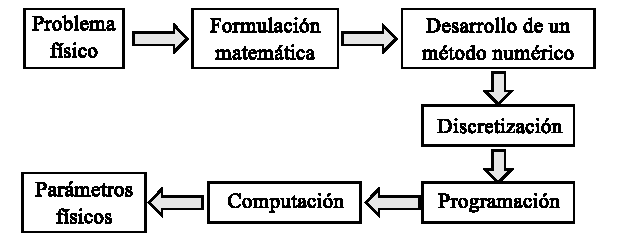
\includegraphics[scale=1]{basic_spanish.pdf}
	\caption{Basado en un esquema del libro ``Theory and computation of electromagnetic fields'' \cite{Jin2010}.}
	\end{figure}
	}	
	\subsection{Estado del arte}
	\frame{
	\frametitle{Sobre las aplicaciones de la simulación en EM}
	\begin{figure}
	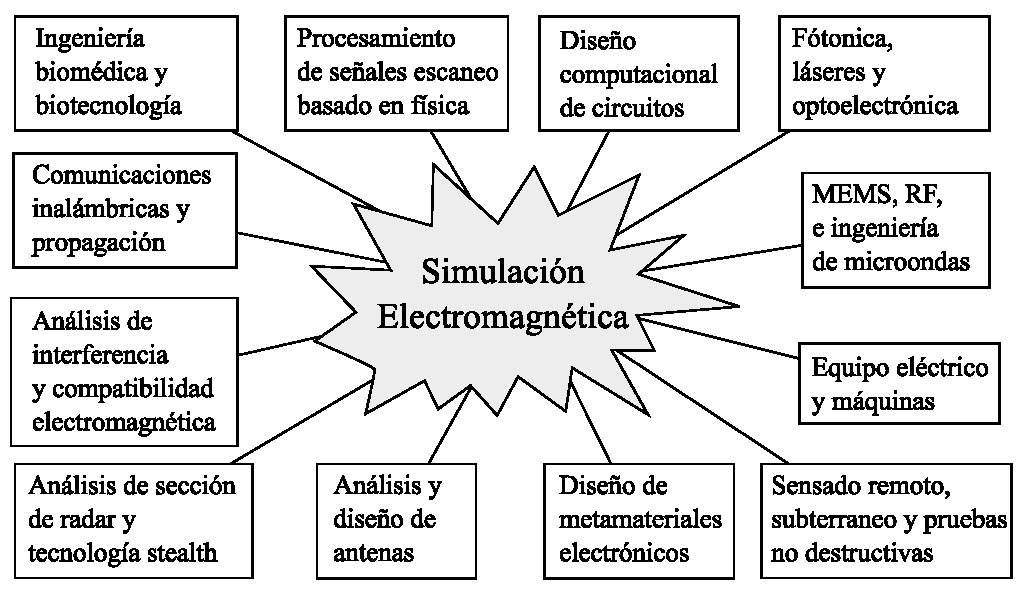
\includegraphics[scale=0.5]{EM_simulation_applications_spanish.pdf}
	\caption{Basado en un esquema del libro ``Theory and computation of electromagnetic fields'' \cite{Jin2010}.}
	\end{figure}
	}
	\frame{
	\frametitle{Estado del arte}
	Antenas sobre substratos hechos a partir de cristales fotónicos tomado de Brown y Yablanovich \cite{E.R.Brown1993a}:
	\note{Los cristales fotónicos como substrato permiten que l radiación de la antena sea dirigida exclusivamente hacia el aire, y no quede atrapada dentro del dieléctrico.}
	
	\begin{figure}
	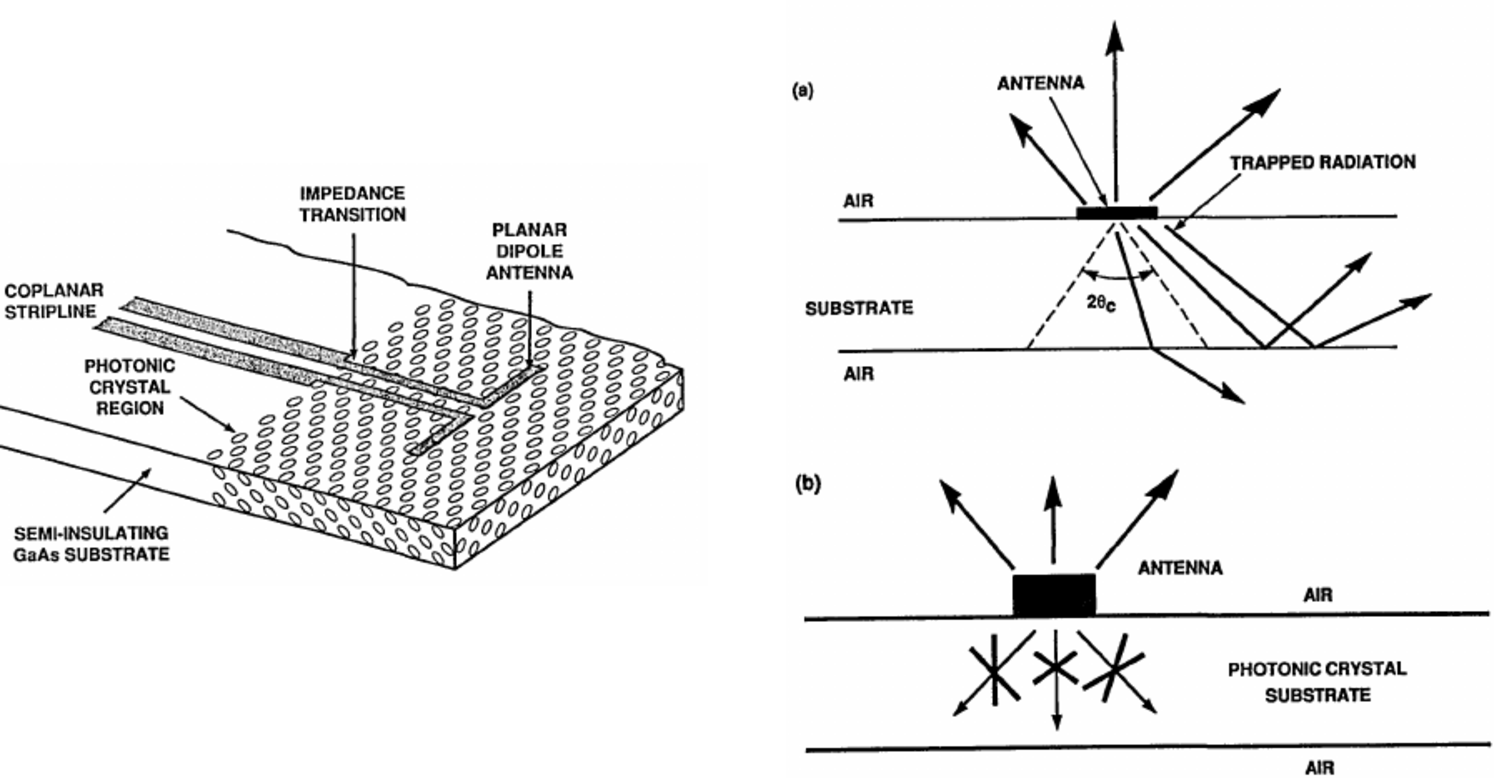
\includegraphics[scale=0.5]{antenna_over_pc.pdf}
	%\caption{Tomado de  \cite{E.R.Brown1993a}}
	\end{figure}
	}
	
	\frame{
	
	Aplicación de cristales fotónicos 1D y 2D para fibras ópticas de nueva generación. Tomado de ``Molding the flow of Light'' Joannopolous \cite{Joannopoulos2008}.
	\vskip15pt
	\begin{figure}
	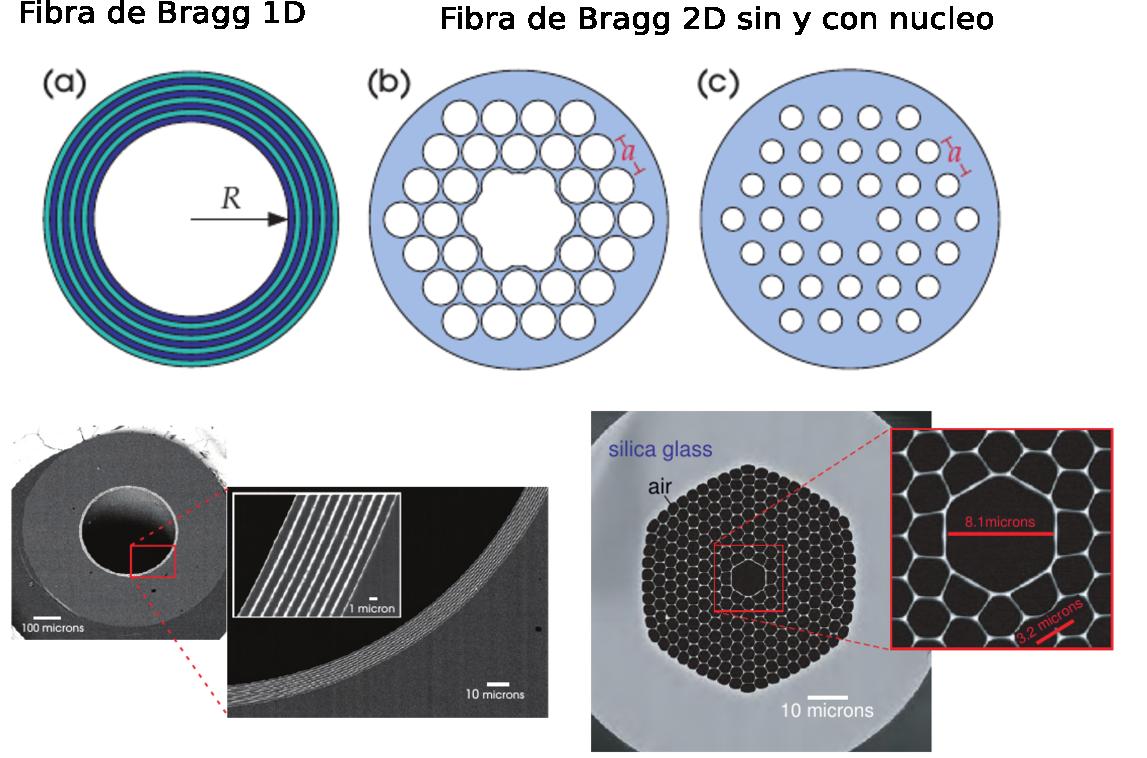
\includegraphics[scale=0.5]{bragg_fibers.pdf}
	%\caption{Tomado de  \cite{E.R.Brown1993a}}
	\end{figure}
	\note{ http://www.nrl.navy.mil/techtransfer/fs.php?fs_id=97}	
	}
	
	\frame{
	La selectividad de los cristales fotónicos ha sido aprovechada por Pervez y Cheng para el desarrollo de espectrómetros ópticos de bajo costo \cite{Pervez2010}.
	\vskip15pt
	\begin{figure}
	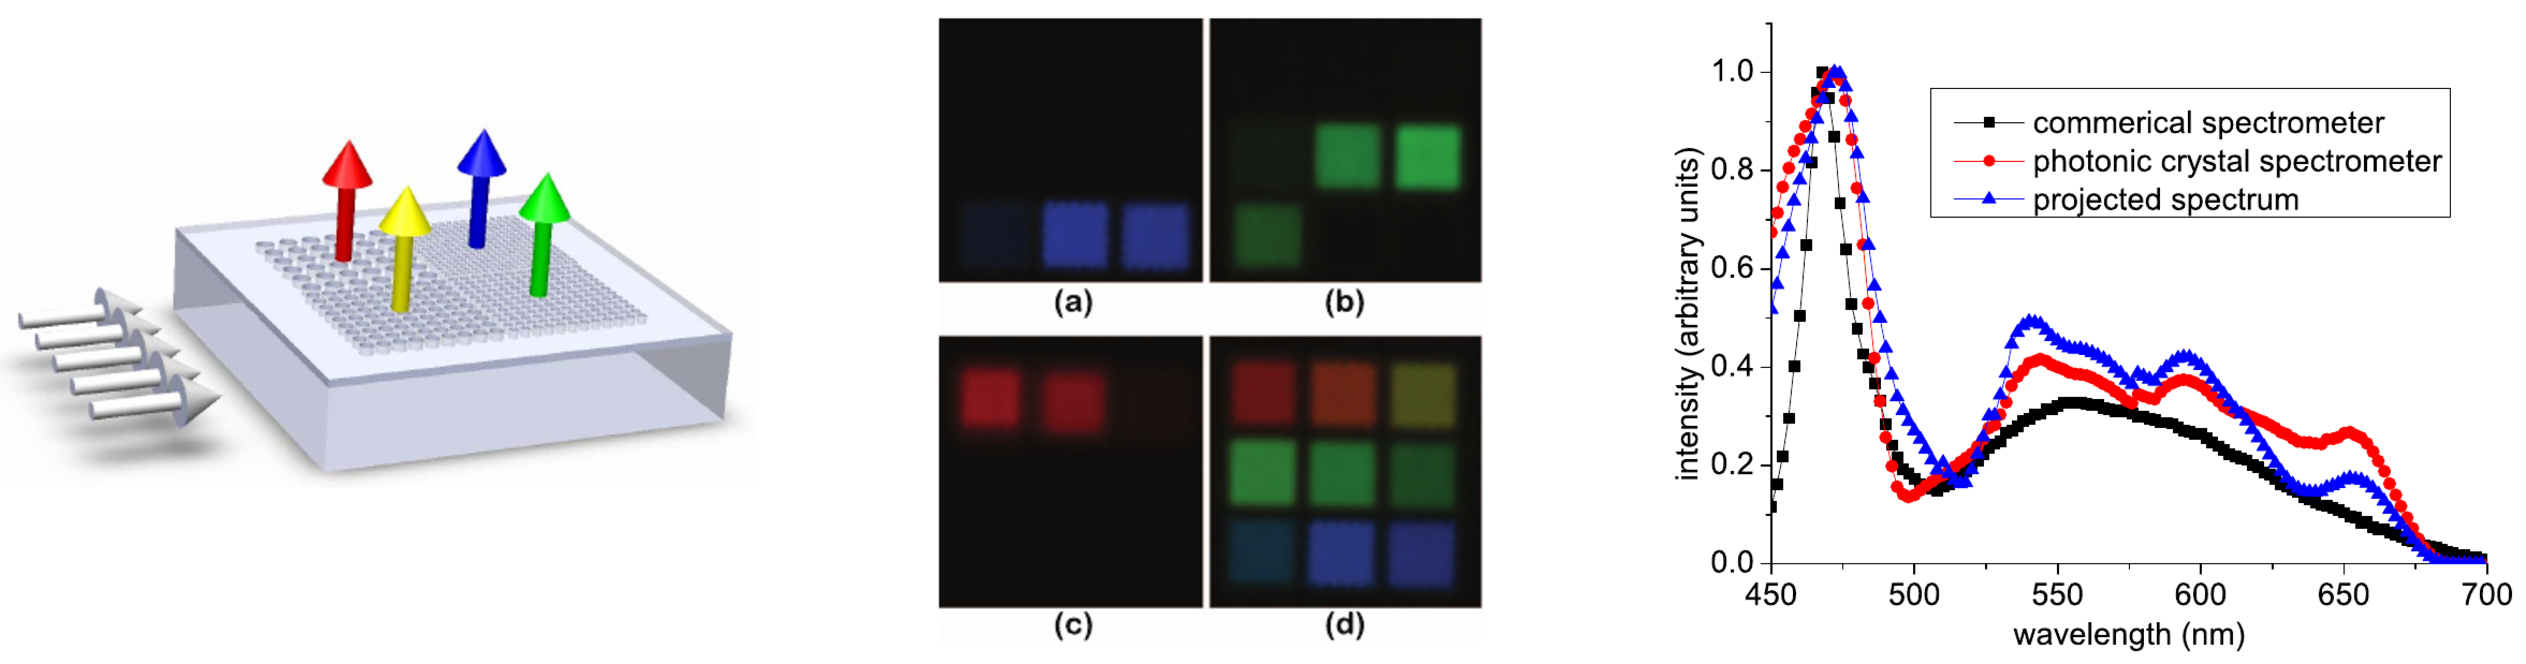
\includegraphics[scale=0.25]{spectrometer.pdf}
	\end{figure}
	}	
	
	\frame{
	\begin{columns}
		\begin{column}{0.4\textwidth}
	Beggs y White desarrollaron acoples con guías de onda hechas a partir de cristales fotónicos que permiten hacer \textit{swicheo} óptico por medio del efecto termo-óptico \cite{beggsdesign}
		\end{column}
		\begin{column}{0.5\textwidth}
			\begin{figure}
			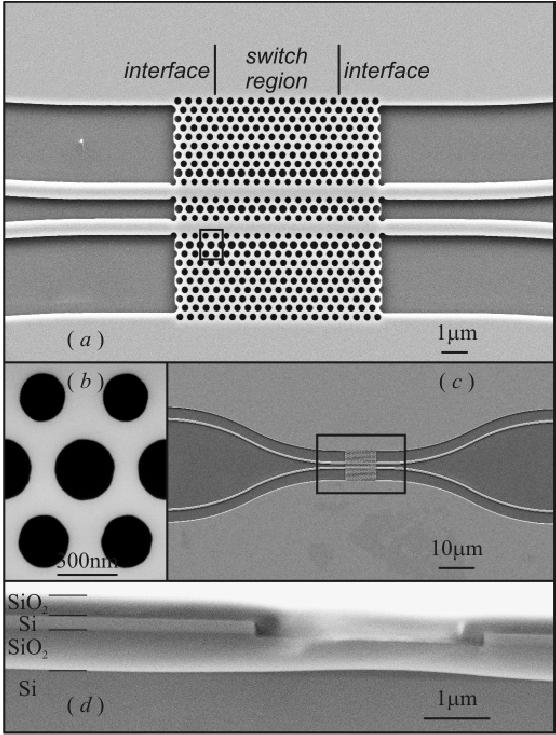
\includegraphics[scale=0.25]{swiche.jpg}
			\end{figure}
			\end{column}
	\end{columns}
	}
	\frame{
	Acoplamiento de puntos cuánticos con cavidades ópticas para procesamiento de información \cite{AndreiFaraon2008}. El estado del sistema se cambia a través de láseres, y la señal que llega a la cavidad está acoplada al estado cuántico del punto.
	\vskip15pt
	\note{Fig. 2. Schematic showing the operation of the device. A heating laser is used to control the
device temperature thus changing the resonance frequency of the cavity and the quantum
dots coupled to it [12]. A probe laser is injected into the cavity from the top. The cavity field
couples to the waveguide mode and then it is scattered from the grating outcoupler into the
collection lens. A pinhole is used to collect only the output scattered by the grating. Using
this device, the transmission function of the cavity can be analyzed for different frequencies
of the resonator, quantum dot and probe laser.
}
	\begin{figure}
	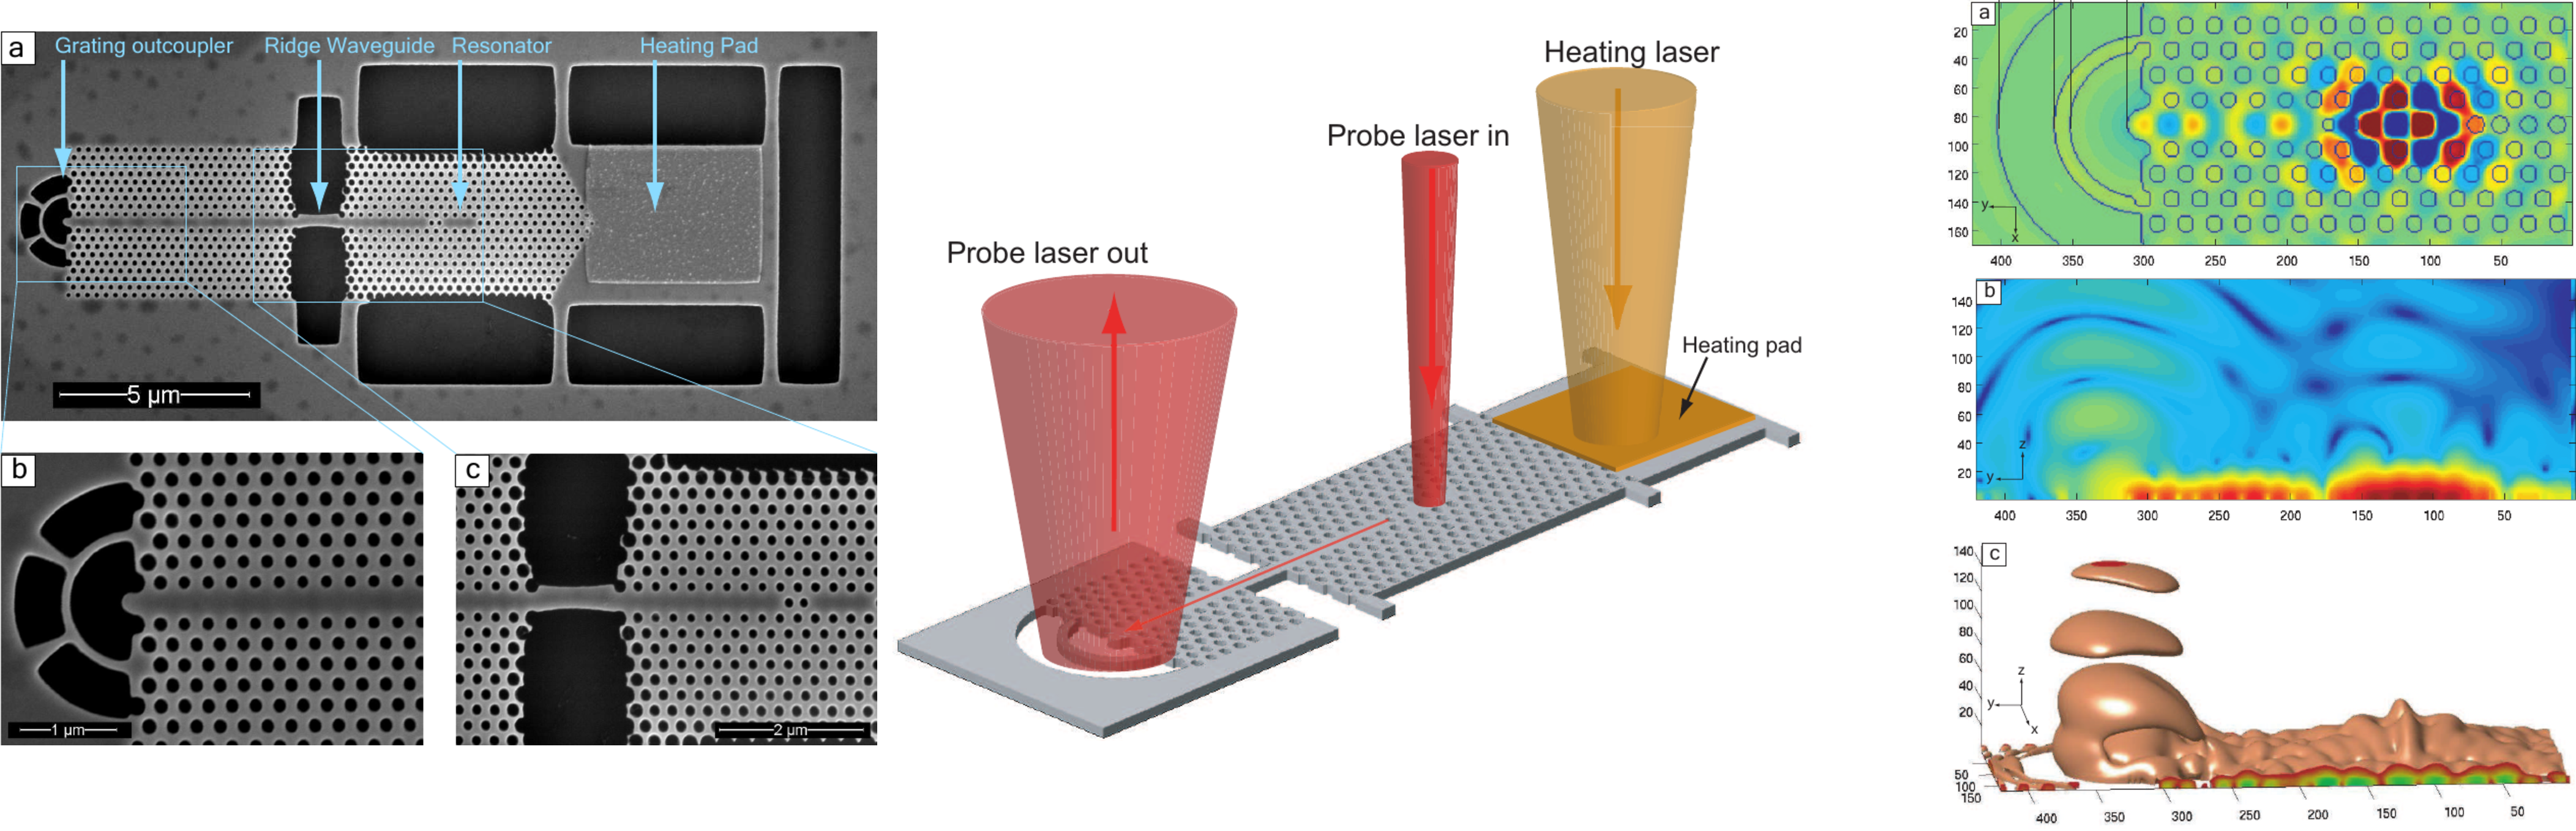
\includegraphics[scale=0.15]{quantum_device.pdf}
	\end{figure}	
	}
\section{Marco Teórico}

	\subsection{La física detrás de un cristal fotónico}
	
	\frame{
	\frametitle{La ecuación de onda}
	\note{Se busca desacoplar las ecuaciones de Faraday
	y Ampere}
	\begin{block}{Ecuación de onda para los campos 
$\mathbf{E}$ y $\mathbf{H}$}
	\small
	Si los vectores de polarización y magnetización no varían con el tiempo:
\begin{align*}
&\nabla\times\nabla\times \mathbf{E} = -\bar{\bar{\mu}}\cdot \left[ \bar{\bar{\epsilon}}\cdot\frac{\partial^2 \mathbf{E}}{\partial t^2} + \frac{\partial \mathbf{J}}{\partial t} \right] \enspace \\
&\nabla\times\nabla\times \mathbf{H} = -\bar{\bar{\epsilon}}\cdot  \bar{\bar{\mu}}\cdot\frac{\partial^2 \mathbf{H}}{\partial t^2} + \nabla\times\mathbf{J} \enspace .
\end{align*}
	\end{block}
	\pause
	\begin{block}{Ecuaciones de Helmholtz}
	\small
	Usando la identidad vectorial  $\nabla\times\nabla\times \mathbf{A} = \nabla(\nabla\cdot\mathbf{A}) - \nabla^2 \mathbf{A}$, y asumiendo que no hay fuentes, tenemos las ecuaciones de Helmholtz para los campos eléctrico y magnético.
	\begin{align*}
&\nabla^2 \mathbf{E} = \bar{\bar{\mu}}\cdot\bar{\bar{\epsilon}}\cdot \frac{\partial^2 \mathbf{E}}{\partial t^2} - \bar{\bar{\mu}}\cdot \frac{\partial \mathbf{J}}{\partial t} \\
&\nabla^2 \mathbf{H} = \bar{\bar{\epsilon}}\cdot\bar{\bar{\mu}}\cdot \frac{\partial^2 \mathbf{H}}{\partial t^2} - \nabla\times \mathbf{J}
\end{align*}
	\end{block}
	}
	
	\frame{
	\small
	\frametitle{Un problema de auto-valores}
	La ecuación de onda armónica se puede tratar como un problema de auto-valores y aprovechar la notación de Dirac para extraer conclusiones sobre las soluciones. El cristal se describe como un problema de la forma:
	
		\begin{equation*}
		\hat{\Theta}\mathbf{E} = \left(\frac{\omega}		{c}\right)^2\mathbf{E}
		\end{equation*} 
		\pause
	Donde 
	\note{El operador $\hat{\Theta}$ está  definido por}
		\begin{equation*}
\hat{\Theta}\mathbf{E}\triangleq \bar{\bar{\mu_r}}^{-1}\nabla\times\nabla\times \mathbf{E}
	\end{equation*}
	\pause
	Al igual que el Hamiltoniano en mecánica cuántica este operador es hermítico, y como tal sus auto-funciones tienen las siguientes propiedades:
	\begin{itemize}
\item Tiene auto valores reales,
\item las auto-funciones son ortogonales entre sí,
\item puede ser obtenido por principios variacionales
\item y se pueden catalogar utilizando propiedades de simetría.
\end{itemize}
	}
	
	\frame{
	\frametitle{Operaciones de traslación}
	En un sistema homogéneo e infinito cualquier punto es equivalente. Es un sistema que es invariante ante traslaciones:
	$$\hat{T}_d\mathbf{E(r)} = \mathbf{E(r-d)}$$
	\begin{figure}
	\animategraphics[autoplay,loop,height=5cm]{0.8}{mediums_}{1}{3}	
	\end{figure}
	\note{Si el sistema tiene simetrías no tenemos cómo diferenciarlo bajo aplicación de operaciones de simetría}
	}
	
	\frame{
	\frametitle{Traslaciones discretas}
	\centering
	\begin{align*}
&r' = r+u_1a_1+u_2a_2
& \hat{T}_{r'}\mathbf{E(r)} = \mathbf{R(r-r')} 
\end{align*}
\pause
	\begin{figure}
	\animategraphics[autoplay,loop,height=5cm]{1}{trans2_}{0}{5}	
	\end{figure}
	}
	
	\frame{
	\frametitle{Condición de Bloch}
	La solución general es una combinación lineal de ondas planas:
	\begin{align*}
\mathbf{E(x,y)}_{k_x,k_y} &= e^{i\vec{k}_x x}e^{i\vec{k}_y y}\sum_{m,n}C_{m,n}e^{imb_1x}e^{imb_2y}\\
\mathbf{E(r)}_{\vec{k}} &= e^{i\vec{k}\cdot r} \mathbf{u}_{\vec{k}}(\mathbf{r})
	\end{align*}
	\pause
	\begin{align*}
\mathbf{E(r+R)}_{\vec{k}} &= e^{i\vec{k}\cdot (\mathbf{r+R})} \mathbf{u}_{\vec{k}}(\mathbf{r+R})\\
\mathbf{E(r+R)}_{\vec{k}} &= e^{i\vec{k}\cdot \mathbf{R}}e^{i\vec{k}\cdot \mathbf{r}} \mathbf{u}_{\vec{k}}(\mathbf{r})\\
\mathbf{E(\mathbf{r}+R)}_{\vec{k}} &= e^{i\vec{k}\cdot \mathbf{R}}\mathbf{E(\mathbf{r})}_{\vec{k}}
	\end{align*}
	}
	\subsection{Los métodos para simular el fenómeno}
	\frame{
	\frametitle{La paleta de herramientas}
	\begin{figure}
	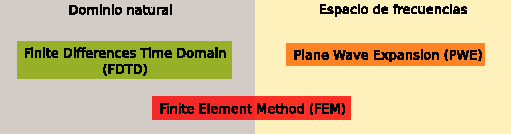
\includegraphics[scale=1.4]{main_methods.pdf}
	\end{figure}
	}
	\frame{	
	\frametitle{La paleta de herramientas}
	\centering
	\begin{figure}
	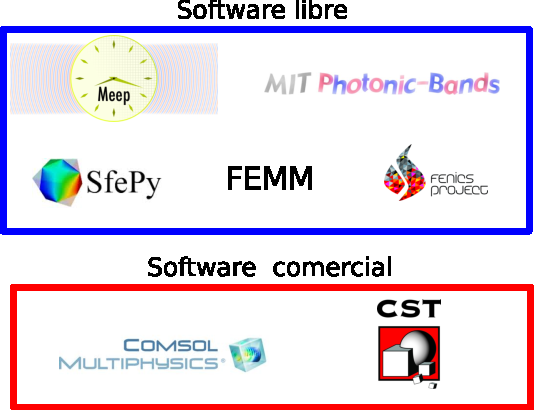
\includegraphics[scale=1]{software.pdf}	
	\end{figure}
	}
	\frame{
	\frametitle{Formulación de Galerkin del método de Elementos finitos.}	
	\begin{itemize}
	\item Es un método de residuos ponderados que aproxima una ecuación diferencial parcial, minimizando un funcional:
 	$$\mathcal{L}(u) = f$$
 	\pause
 	$$\mathcal{R} = \mathcal{L}(u')-f$$
 	\pause
	$$\int w \mathcal{R}(u') = 0$$
	\pause
	\item Se diferencia de otros métodos porque la función de ponderación tiene la misma base que las funciones de aproximación.
	\end{itemize}
	}	
	\frame{
	\frametitle{Discretización}
	%\only<3-4>{\frametitle{Discretización Vectorial}}
		
	\begin{align*}
	\mathbf{E} &= \sum_{el=1}^{N_{el}}\mathbf{E}^{el}
	&\mathbf{E}^{el} = \sum_{i =1}^N E_i^{el}h_i^{el}
		\end{align*}
		
%		\only<3>{\begin{align*}
%E(x,y)_x\approx \sum_{i:\ n_x \in \eta_D} h_i E_i^x+\sum_{i:\ n_x \in \eta\setminus\eta_D} h_i E_i^x \\
%E(x,y)_y\approx \sum_{i:\ n_y \in \eta_D}h_iE_i^y+
%\sum_{i:\ n_x \in \eta\setminus\eta_D}h_iE_i^y
%\end{align*}}
%		\only<4>{\begin{align*}
%W(x,y)_x\approx \sum_{i:\ n_x \in \eta_D} h_i W_i^x+\sum_{i:\ n_x \in \eta\setminus\eta_D} h_i W_i^x \\
%W(x,y)_y\approx \sum_{i:\ n_y \in \eta_D}h_iW_i^y+
%\sum_{i:\ n_x \in \eta\setminus\eta_D}h_iW_i^y
%\end{align*}}
		\begin{figure}
		\centering
		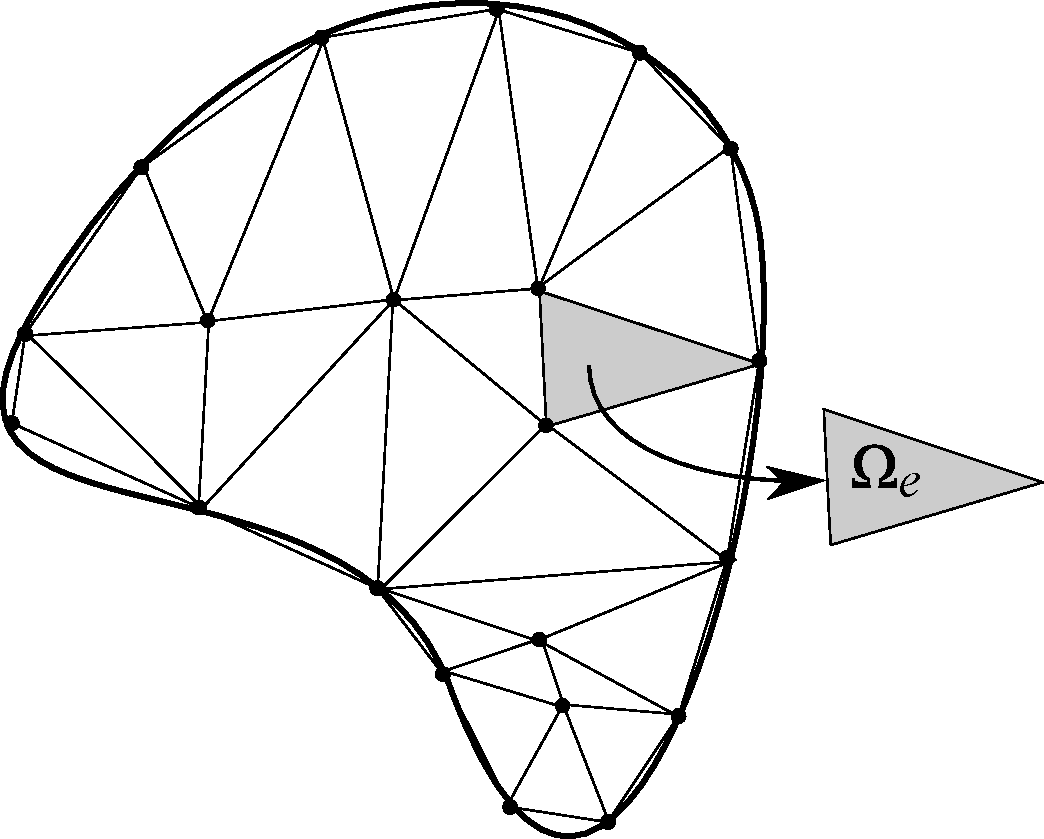
\includegraphics[scale=0.3]{dominio_discreto.pdf}
		\caption{\tiny Dominio discretizado, definido por un conjunto de elementos y sus nodos \cite{Guarin2012}}.
		\end{figure}	
	}
	\begin{frame}
	\frametitle{Un sistema de ecuaciones lineales}
	
	La discretización del dominio hace que la ecuación de onda se pueda definir como un problema discreto representado por un sistema de ecuaciones:
	\begin{equation*}
^{\setminus D}\left[\left(\mathbb{A}-\mathbb{M}\right)\vec{E}= -\vec{d}-\vec{q}-\vec{f}\right]
\end{equation*}
	\pause
	Que proviene de partir el funcional en operadores
	\begin{figure}
	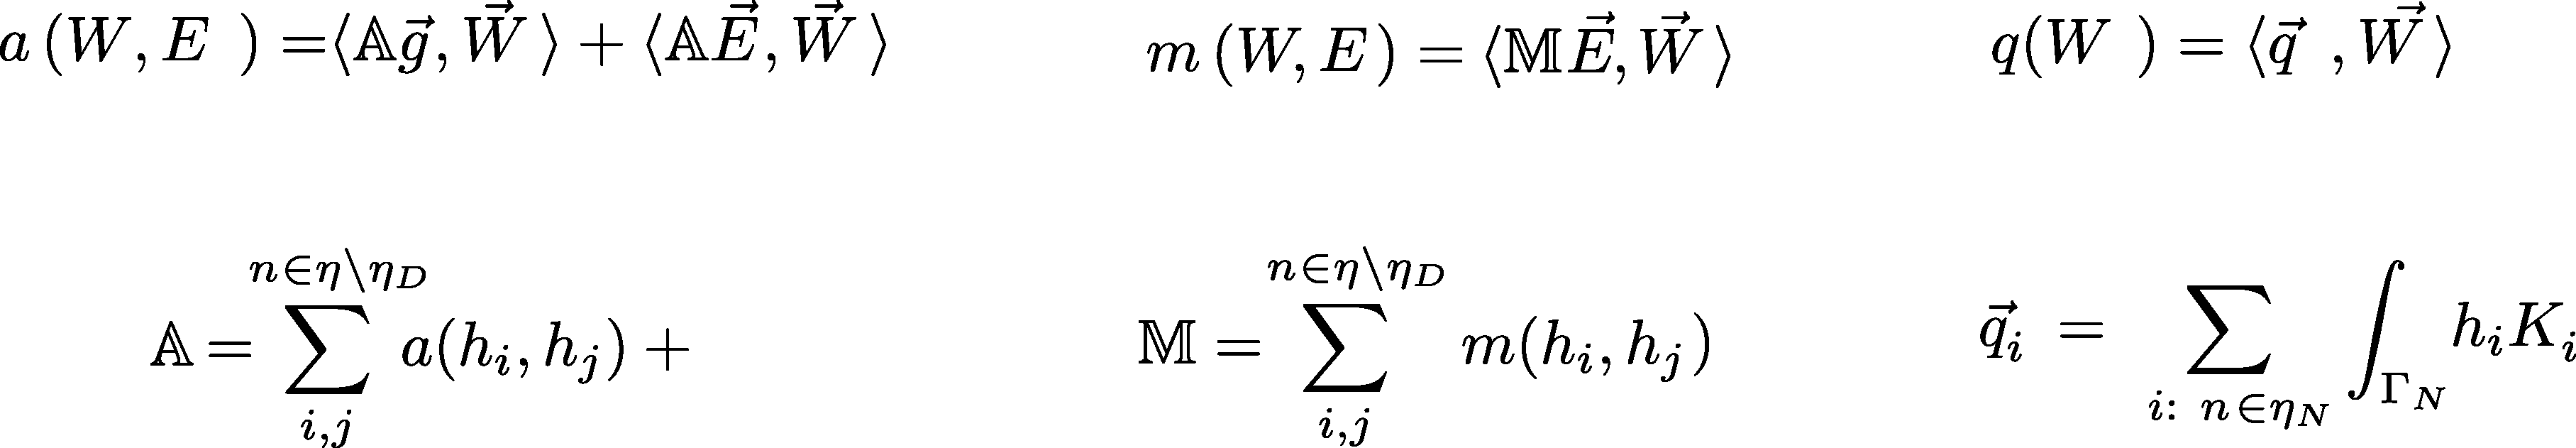
\includegraphics[scale=0.18]{matrices_3.pdf}
	\end{figure}		
%	\begin{figure}
%	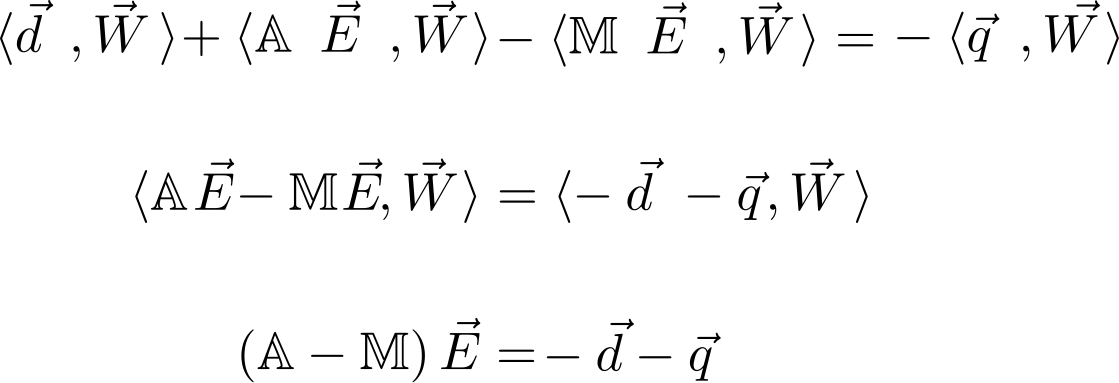
\includegraphics[scale=0.2]{matrices_4.png}
%	\end{figure}		
	
%	\only<2>{
%	Las funciones base y las funciones de prueba discretas se ingresan en la forma abstracta del funcional:	
	
%	\only<2>{
%	Los operadores del funcional se interpretan como productos interiores de vectores discretos:
%	\begin{figure}
%	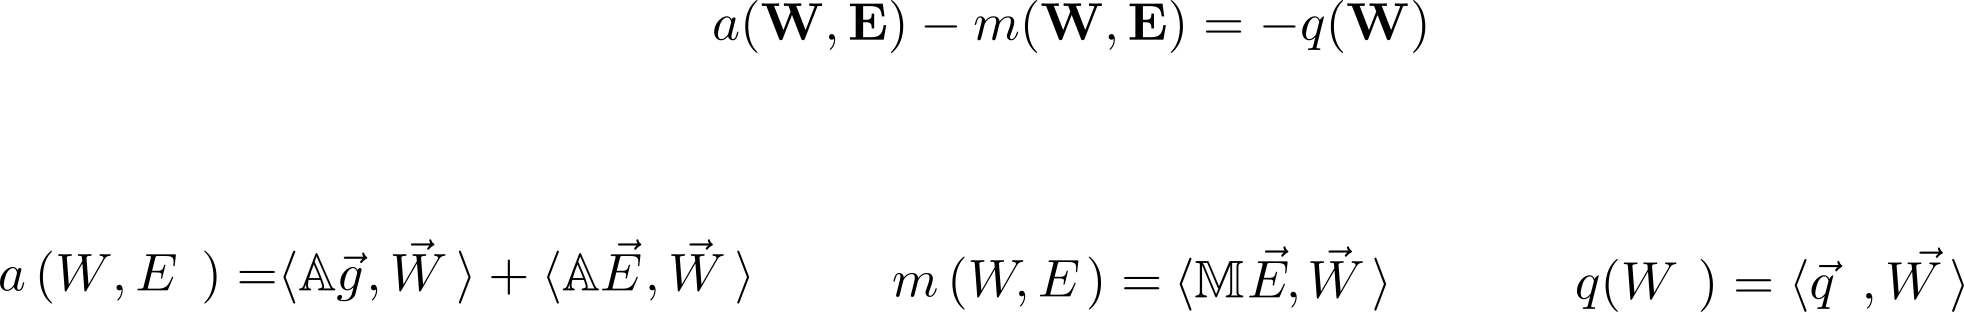
\includegraphics[scale=0.15]{matrices_2.png}
%	\end{figure}		
%	}
%	\only<2>{
%	Al actuar sobre elementos discretos los operadores también se discretizan:
%	\begin{figure}
%	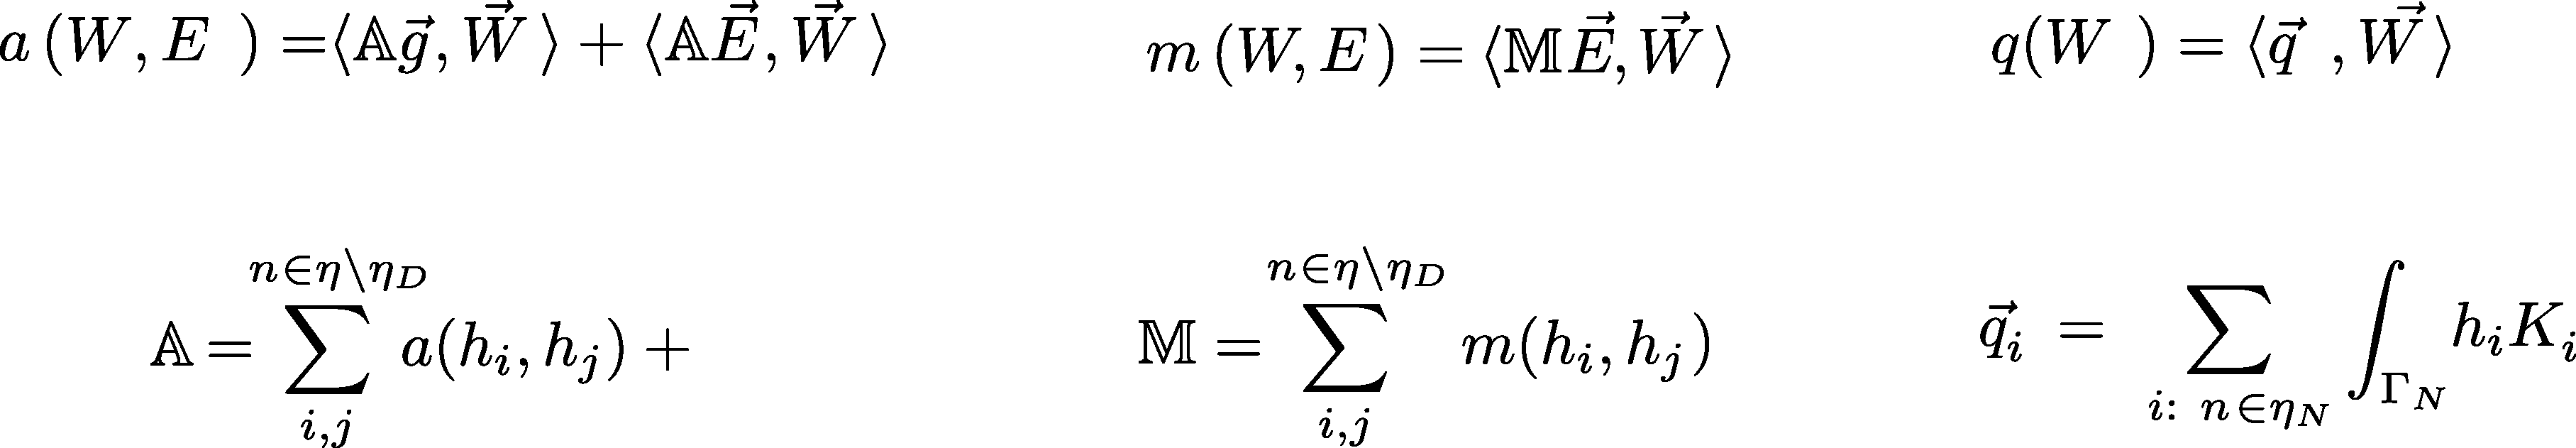
\includegraphics[scale=0.18]{matrices_3.pdf}
%	\end{figure}		
%	}
%	
	\end{frame}	
	\frame{
	\frametitle{La forma débil del problema}
	\begin{columns}
		\column{0.3\textwidth}
			\uncover<1->{
			\begin{figure}
			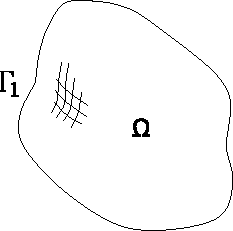
\includegraphics[scale=0.8]{dominio.pdf}
			\end{figure}}
		\column{0.7\textwidth}
				\begin{block}{\small Forma débil con condiciones de frontera.}
				\small
				\begin{equation*}
				\int_{\Omega} \bar{\bar{\mu_r}}^{-1}\nabla\times \mathbf{E}\cdot \nabla\times\mathbf{W}
				-\int_{\Omega}k_0^{2}\mathbf{W}\cdot \bar{\bar{\epsilon_r}}\cdot \mathbf{E}
				=- \int_{\Gamma_N} \mathbf{W} \cdot\mathbf{K}_N 
				\end{equation*}
			\end{block}
			\begin{block}{\small Funcional a minimizar}
			\scriptsize
				\begin{equation*}
			\int_{\Omega}\mathbf{W}\cdot\left[ \nabla\times\ \left(\bar{\bar{\mu_r}}^{-1}\nabla\times \mathbf{E} \right) - k_0^{2}\bar{\bar{\epsilon_r}}\cdot \mathbf{E}\right]= - ik_0Z_0 \int_{\Omega} \mathbf{W}\cdot\mathbf{J} 
				\end{equation*}
			\end{block}
%			\pause
%			\begin{block}{\small Forma débil}
%				\tiny
%				\begin{align*}
%\int_{\Omega} \bar{\bar{\mu_r}}^{-1}\nabla\times \mathbf{E}\cdot \nabla\times\mathbf{W}
%-\int_{\Omega}k_0^{2}\mathbf{W}\cdot \bar{\bar{\epsilon_r}}\cdot \mathbf{E}
%&+&\\ \int_{\Gamma_N} \mathbf{W} \cdot
% \left(\hat{n}\times\bar{\bar{\mu_r}}^{-1}
%\nabla\times\mathbf{E}\right)
%&=& -ik_0Z_0 \int_{\Omega} \mathbf{W}\cdot\mathbf{J}
%				\end{align*}
%			\end{block}
%			\pause
	\end{columns}
	}
	
	\frame{
	\frametitle{Elementos y funciones de interpolacion}
		\begin{figure}
		\centering
		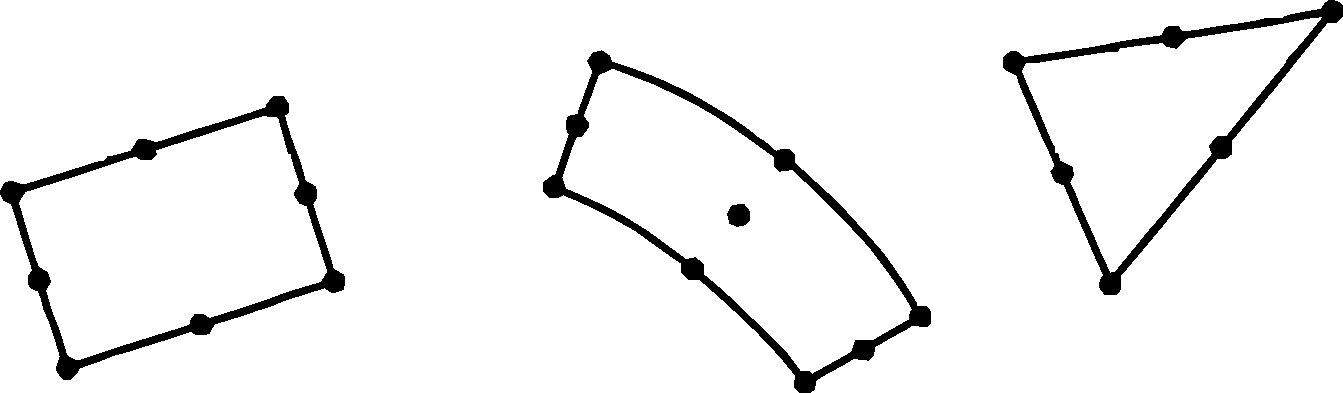
\includegraphics[scale=0.4]{two_dim_elem.pdf}
		\caption{Elementos 2D comúnmente usados en electromagnetismo.\cite{Bathe1996}}
		\end{figure}		
		\pause
		\begin{figure}
		\centering
		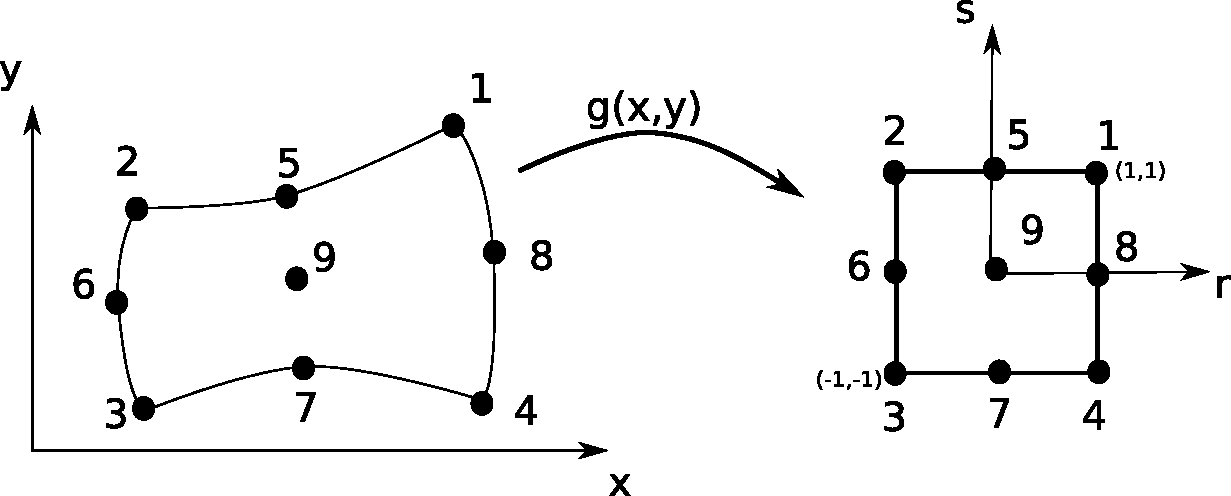
\includegraphics[scale=0.3]{./img/2D_gen_elem.pdf}
		\caption{Mapeo a elementos isoparamétricos}
		\end{figure}
	}
	
	\frame{
	\frametitle{Elementos y funciones de interpolacion}
	\begin{figure}
	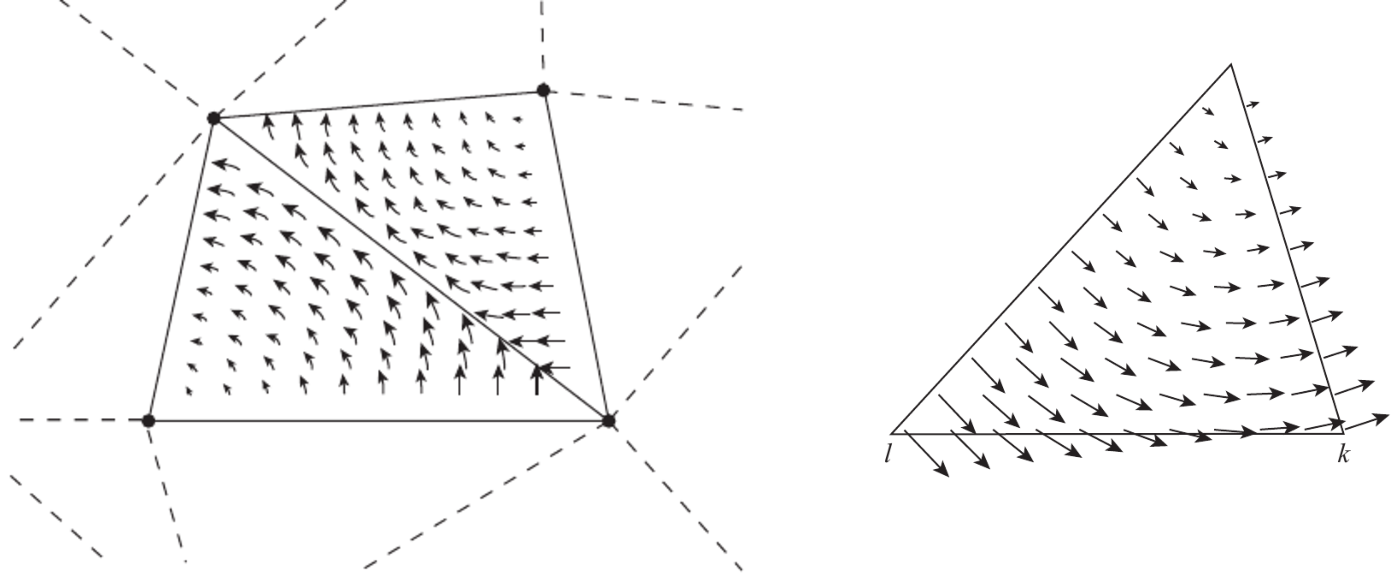
\includegraphics[scale=0.5]{edge_element.pdf}
	\caption{Elementos triangulares de borde tomados de Jian \cite{Jin2010}}
	\end{figure}
	}
	
	\frame{
	\frametitle{Diferencias centradas y formulación explícita}
	La misma formulación se puede hacer para problemas no armónicos:
	\begin{equation*}
\mathbb{A}\left\lbrace \mathcal{E} \right\rbrace- \mathbb{M}\frac{\partial^2\left\lbrace\mathcal{E} \right\rbrace}{\partial t^2} = -\left\lbrace d \right\rbrace-\left\lbrace q   \right\rbrace
	\end{equation*}
	\pause
	En este caso se usa la aproximación de diferencias finitas centradas para modelar el cambio temporal:
	\begin{equation*}
\ddot{\mathbf{E}}_n = \frac{1}{\delta t^2}\left(\mathbf{E}_{n+1}-2 \mathbf{E}_{n} + \mathbf{E}_{n-1}\right)
	\end{equation*}	
	\begin{equation*}
\frac{1}{\delta t^2} \mathbb{M} \mathbf{E}_{n+1} = - \mathbb{A}\mathbf{E}_n + \frac{1}{\delta t^2}\mathbb{M}\left[2
\mathbf{E}_{n}-\mathbf{E}_{n-1}
\right] 	 
	\end{equation*}
	\note{Mencionar matrices de masa diagonales}	
	}
\section{Implementación}
	\frame{
	\frametitle{ Pasos que se siguieron en el desarrollo de Software}
	\setbeamercovered{transparent}
	\begin{itemize}
	\item<1-> Se parte de unos requerimientos, de uso y funcionalidad,
	\item<2-> y se evalúan alternativas para cumplirlos.
	\item<3-> Abstracción del problema y la estructura del programa.
	\item<4-> Selección de un lenguaje y herramientas acordes a los requerimientos.
	\item<5-> Programación y depuración de las rutinas.	
	\end{itemize}
	\setbeamercovered{invisible}
	\uncover<6->{Adicionalmente: 

	\begin{itemize}
	\item Se debe establecer un sistema de control de cambios,
	\item y generar documentación para los posibles usuarios o desarrolladores.
	\end{itemize}	
	}		
	}
	\subsection{Requerimientos}
	\frame{
	\frametitle{Requerimientos de PeyeQM}
	\begin{description}
	\item[Modularidad] Diseño de software haciendo uso de componentes independientes o levemente interconectados \cite{Lage1998}. 
	\item[Reusabilidad] La flexibilidad necesaria para que un segmento de código pueda ser usado en contextos distintos sin necesidad de introducir modificaciones.
\item[Extensibilidad] El diseño tiene en consideración el crecimiento de la aplicación.
\item [Multiplataforma] Software que se implementa para operar en múltiples sistemas operativos \cite{PCMag}.
%\item<6->[Readability]  A human judgment of how easy a
%text is to understand. ``The readability of a program is related
%to its maintainability'' \cite{Raymond2008}.
	\item[Libre y abierto] Se quiere que la plataforma, y las herramientas asociadas sean libres de distribuir, copiar, y o modificar.
	\end{description}	
	}
	\subsection{Paradigmas}
	\frame{
	\frametitle{Paradigmas, y alternativas de desarrollo}
	\begin{figure}
	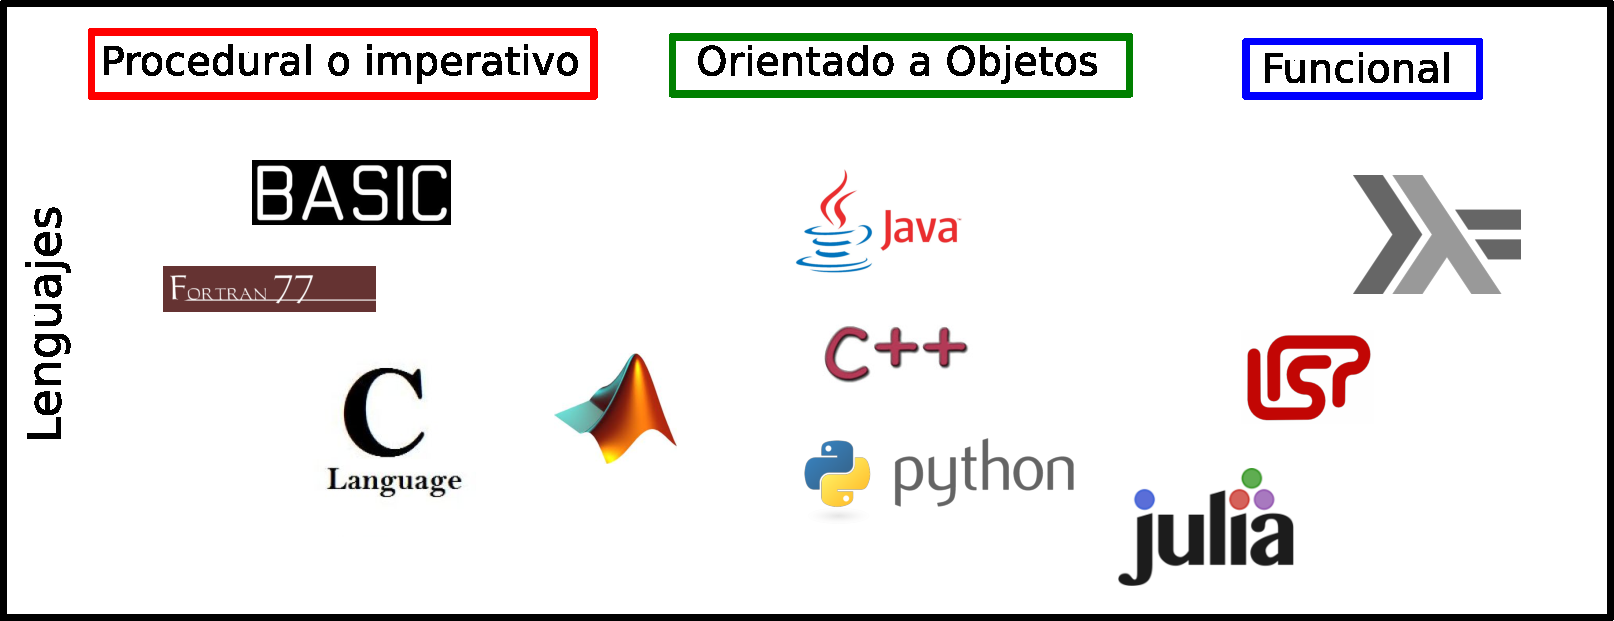
\includegraphics[scale=0.4]{lenguajes.pdf}
	\end{figure}		
	}
	\frame{
	\frametitle{Programación Orientada a Objetos}
		\begin{columns}
		\begin{column}{0.2 \textwidth}
		\shadowbox{Abstracción}
		\note{Con la abstracción se puede lograr modularidad. Podemos crear objetos arbitrarios que poseen características comunes}
		\shadowbox{Encapsulación}
		\shadowbox{Herencia}
		\shadowbox{Polimorfismo}
			\note{Data abstraction In OOP data abstraction is obtained by definition of classes. A class is the
set of common attributes that a general object of a certain kind or class has. For example,
“Banana” class would represent the properties and functionality of bananas in general, such
as being edible, or having potassium. Usage of data abstraction allows us to generalize the
behavior of objects independently of what is their current state (name, value of its attributes).
}
			\end{column}
			\pause
			\begin{column}{0.7 \textwidth}
			Un ejemplo:						
			\begin{figure}
			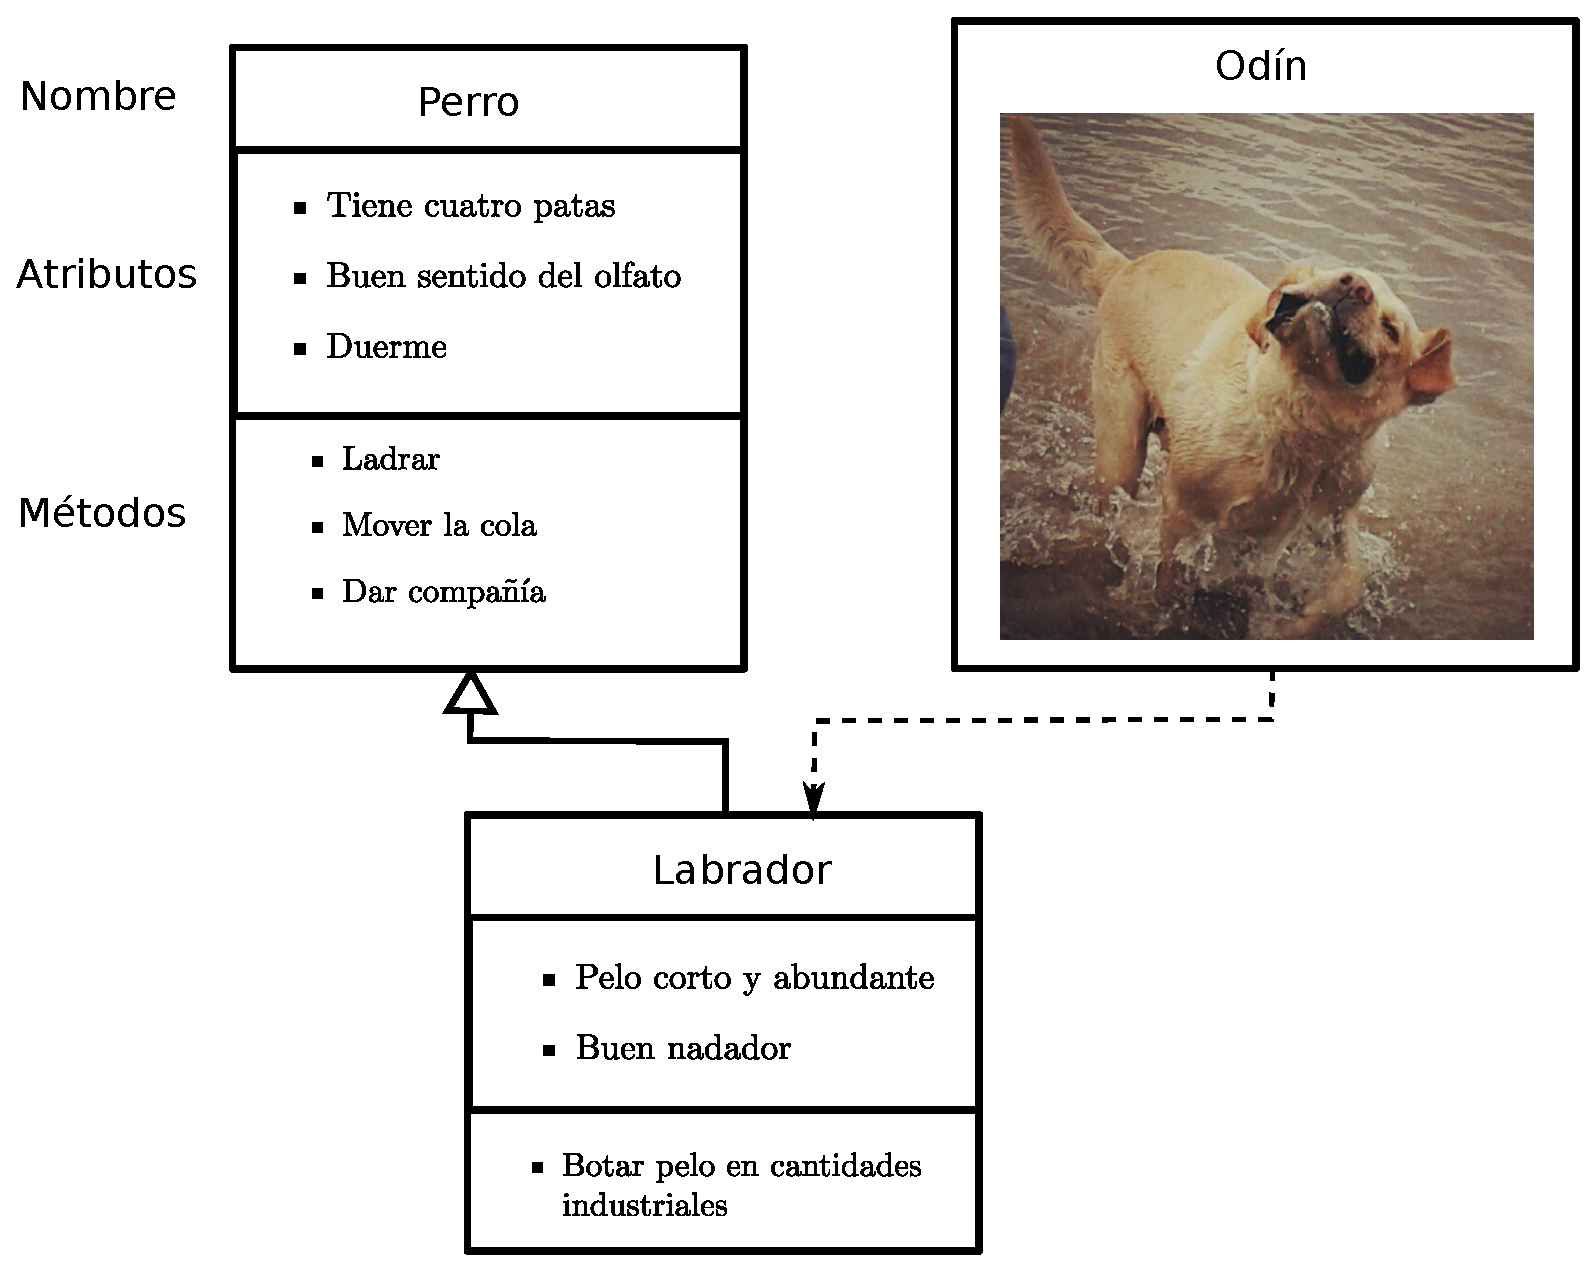
\includegraphics[scale=0.3]{clase_perro.eps}
			\end{figure}
			\end{column}
		\end{columns}
	}	
	\subsection{Herramientas}
	\frame{
	\frametitle{Herramientas}
	\begin{columns}
	\column{0.4\textwidth}
		\begin{block}{Python, Spyder y Scipy}
		\centering
			\begin{figure}
			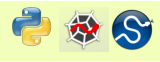
\includegraphics[scale=1.5]{scripting.pdf}	
			\end{figure}
		\end{block}		
		\begin{block}{Gmsh y Paraview}
		\centering
			\begin{figure}
			
\includegraphics[scale=1.5]{post_y_pre_proc.pdf}	
			\end{figure}
		\end{block}	
	\column{0.4\textwidth}
		\begin{block}{Git y Github}
		\centering
			\begin{figure}
			
\includegraphics[scale=1.5]{version_control.pdf}	
			\end{figure}
		\end{block}		
		\begin{block}{Documentación}
		\centering
			\begin{figure}
			
\includegraphics[scale=1]{sphinx.pdf}	
			\end{figure}
		\end{block}	
	\end{columns}
	}
	\subsection{Estructura}
	\frame{
	\frametitle{Estructura de PeyeQM}
		\only<1>{
			\begin{figure}
			\centering
			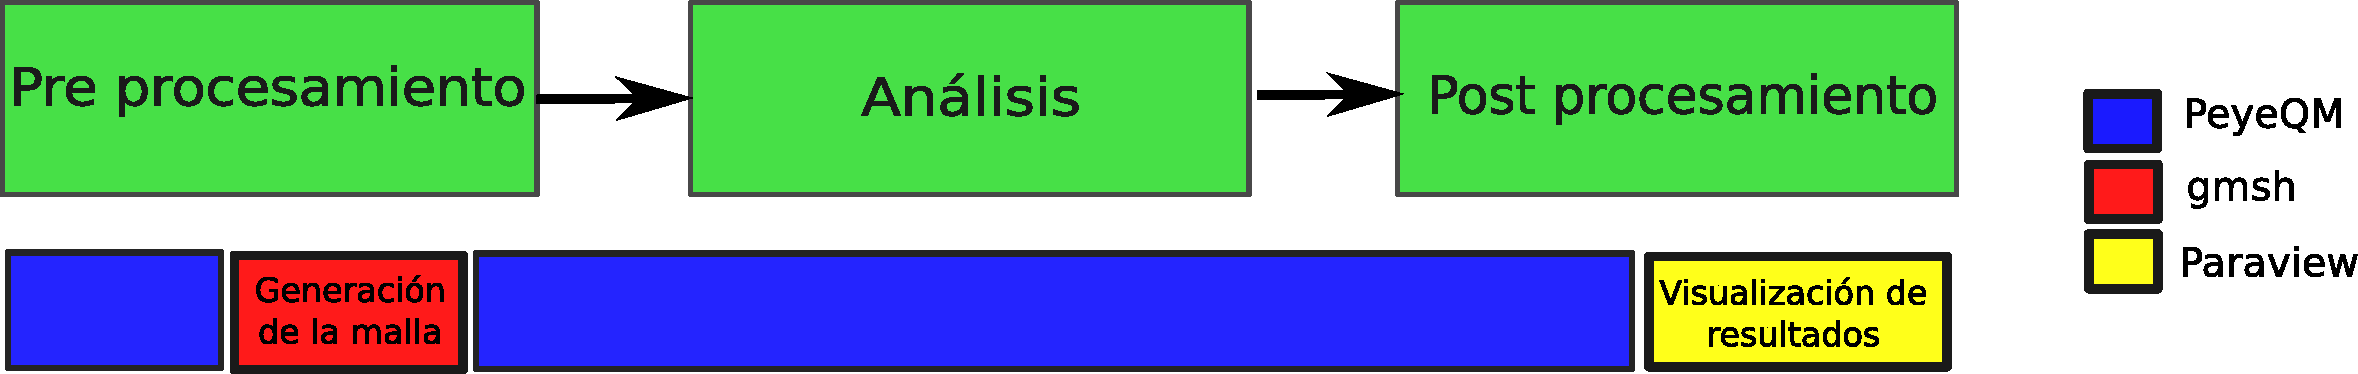
\includegraphics[scale=.3]{stages_comparison_spanish.pdf}
			\caption{Representación de qué parte del proceso de simulación es hecho usando las rutinas de PeyeQM.}
			\end{figure}  	
		}
		\only<2>{
			\begin{figure}[h]
			\centering
			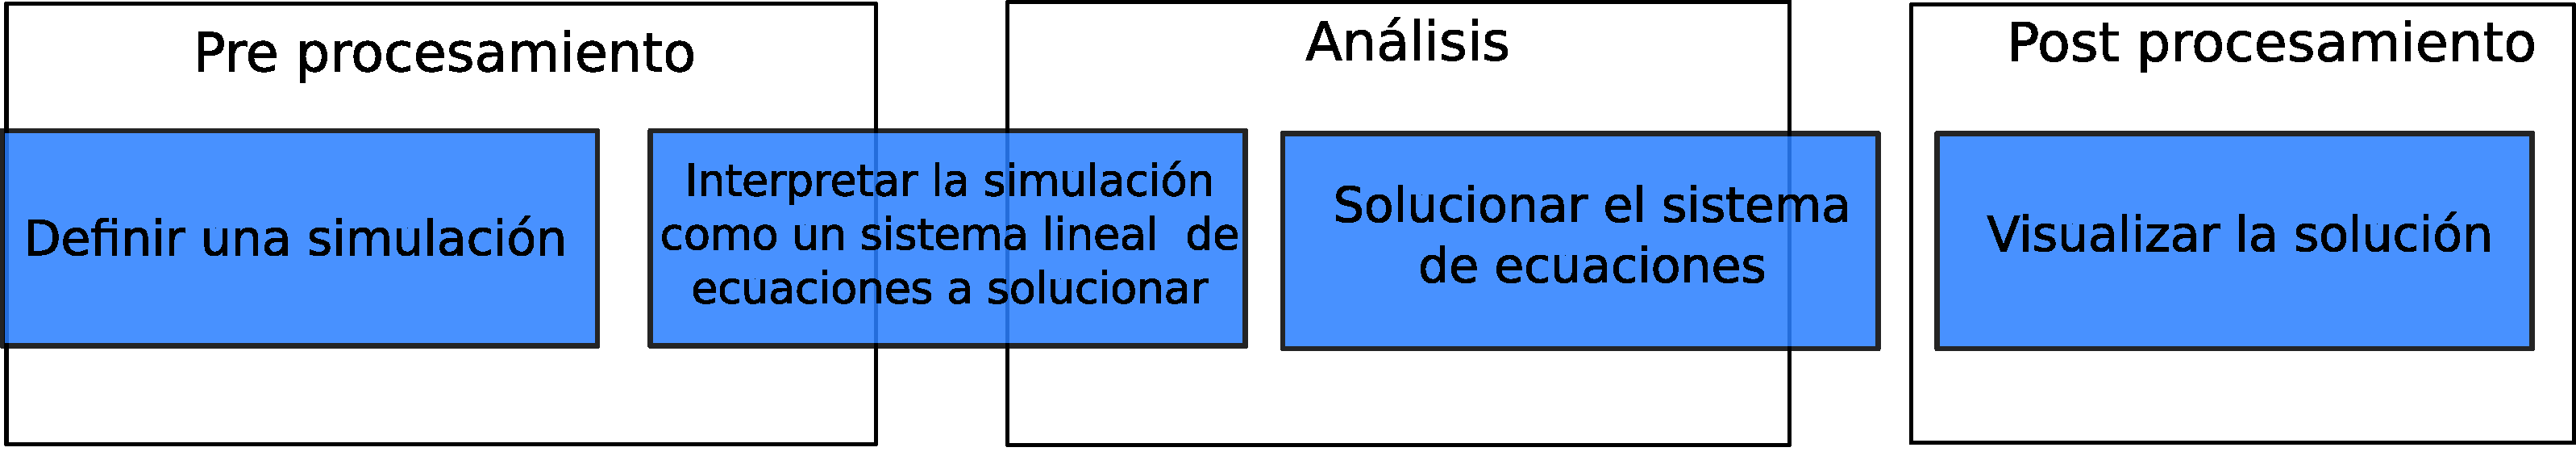
\includegraphics[scale=.22]{stages_abstract_spanish.pdf}
			\caption{Interpretación en PeyeQM de las tres etapas.}
			\end{figure}
		}
		\only<3>{
			\begin{figure}
			\centering
			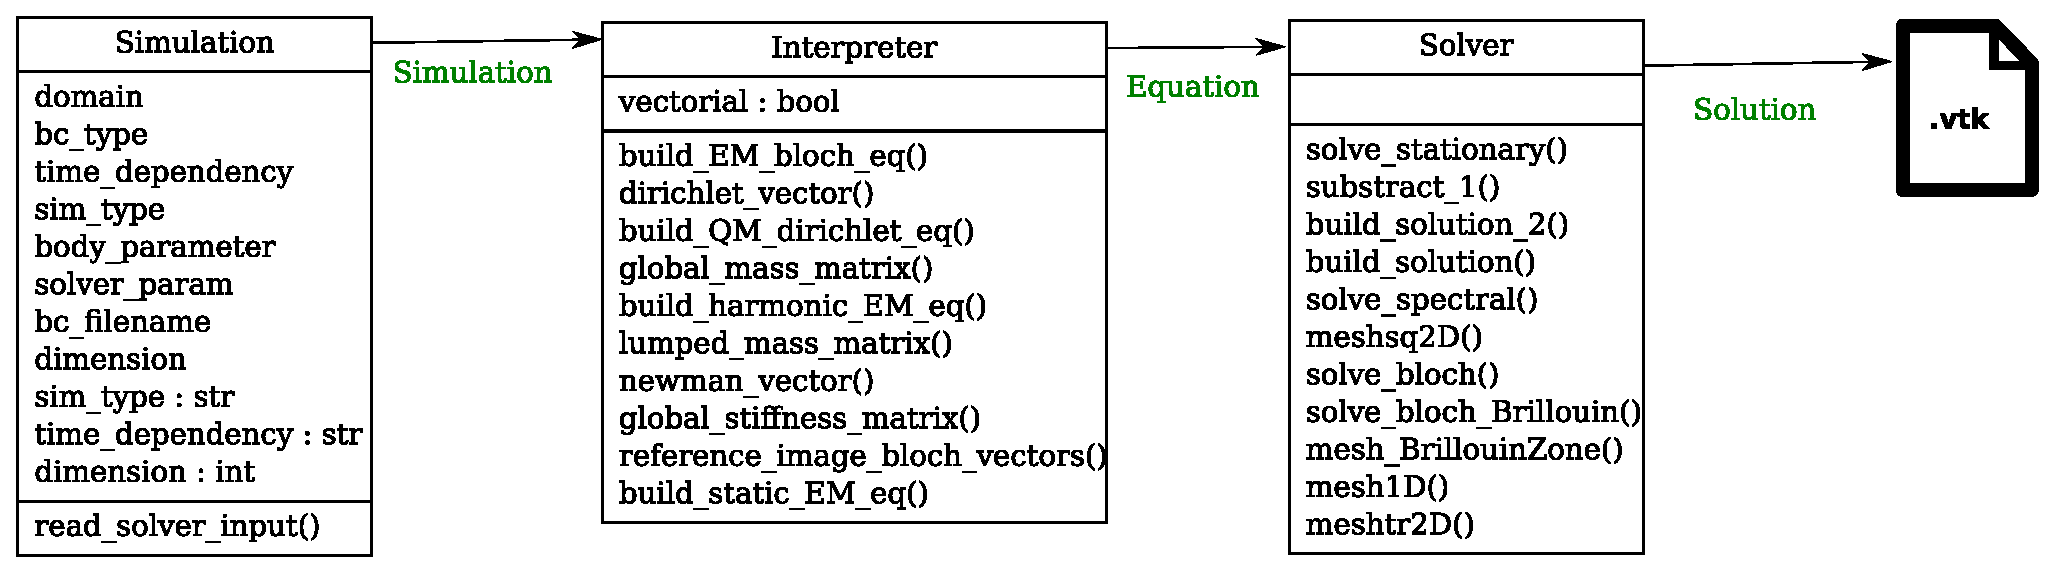
\includegraphics[scale=0.35]{classes_reduced.eps}
			\caption{Diagrama clases superiores.}
			\end{figure}		
		}
		\only<4>{
			\begin{figure}
			\centering
			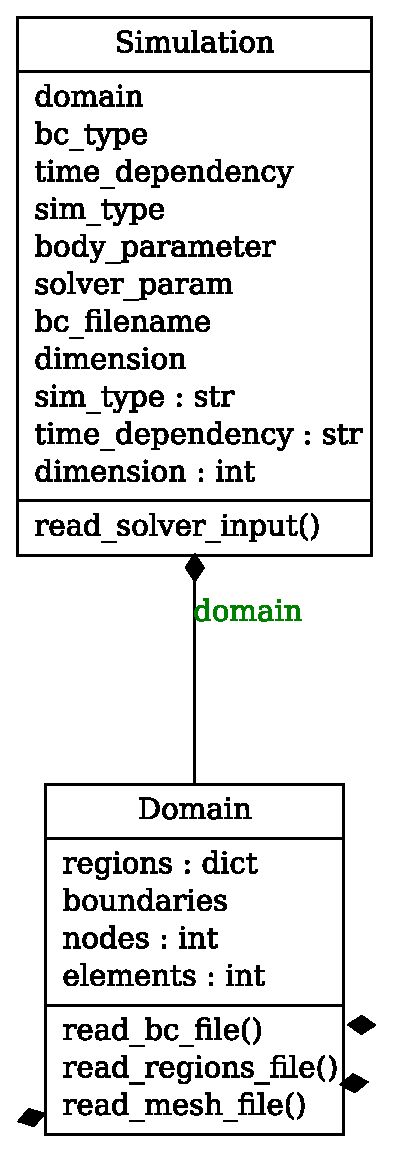
\includegraphics[scale=0.35]{classes_reduced_2.eps}
			\caption{Diagrama de clase Simulation.}
			\end{figure}		
		}
		\only<5>{
			\begin{figure}
			\centering
			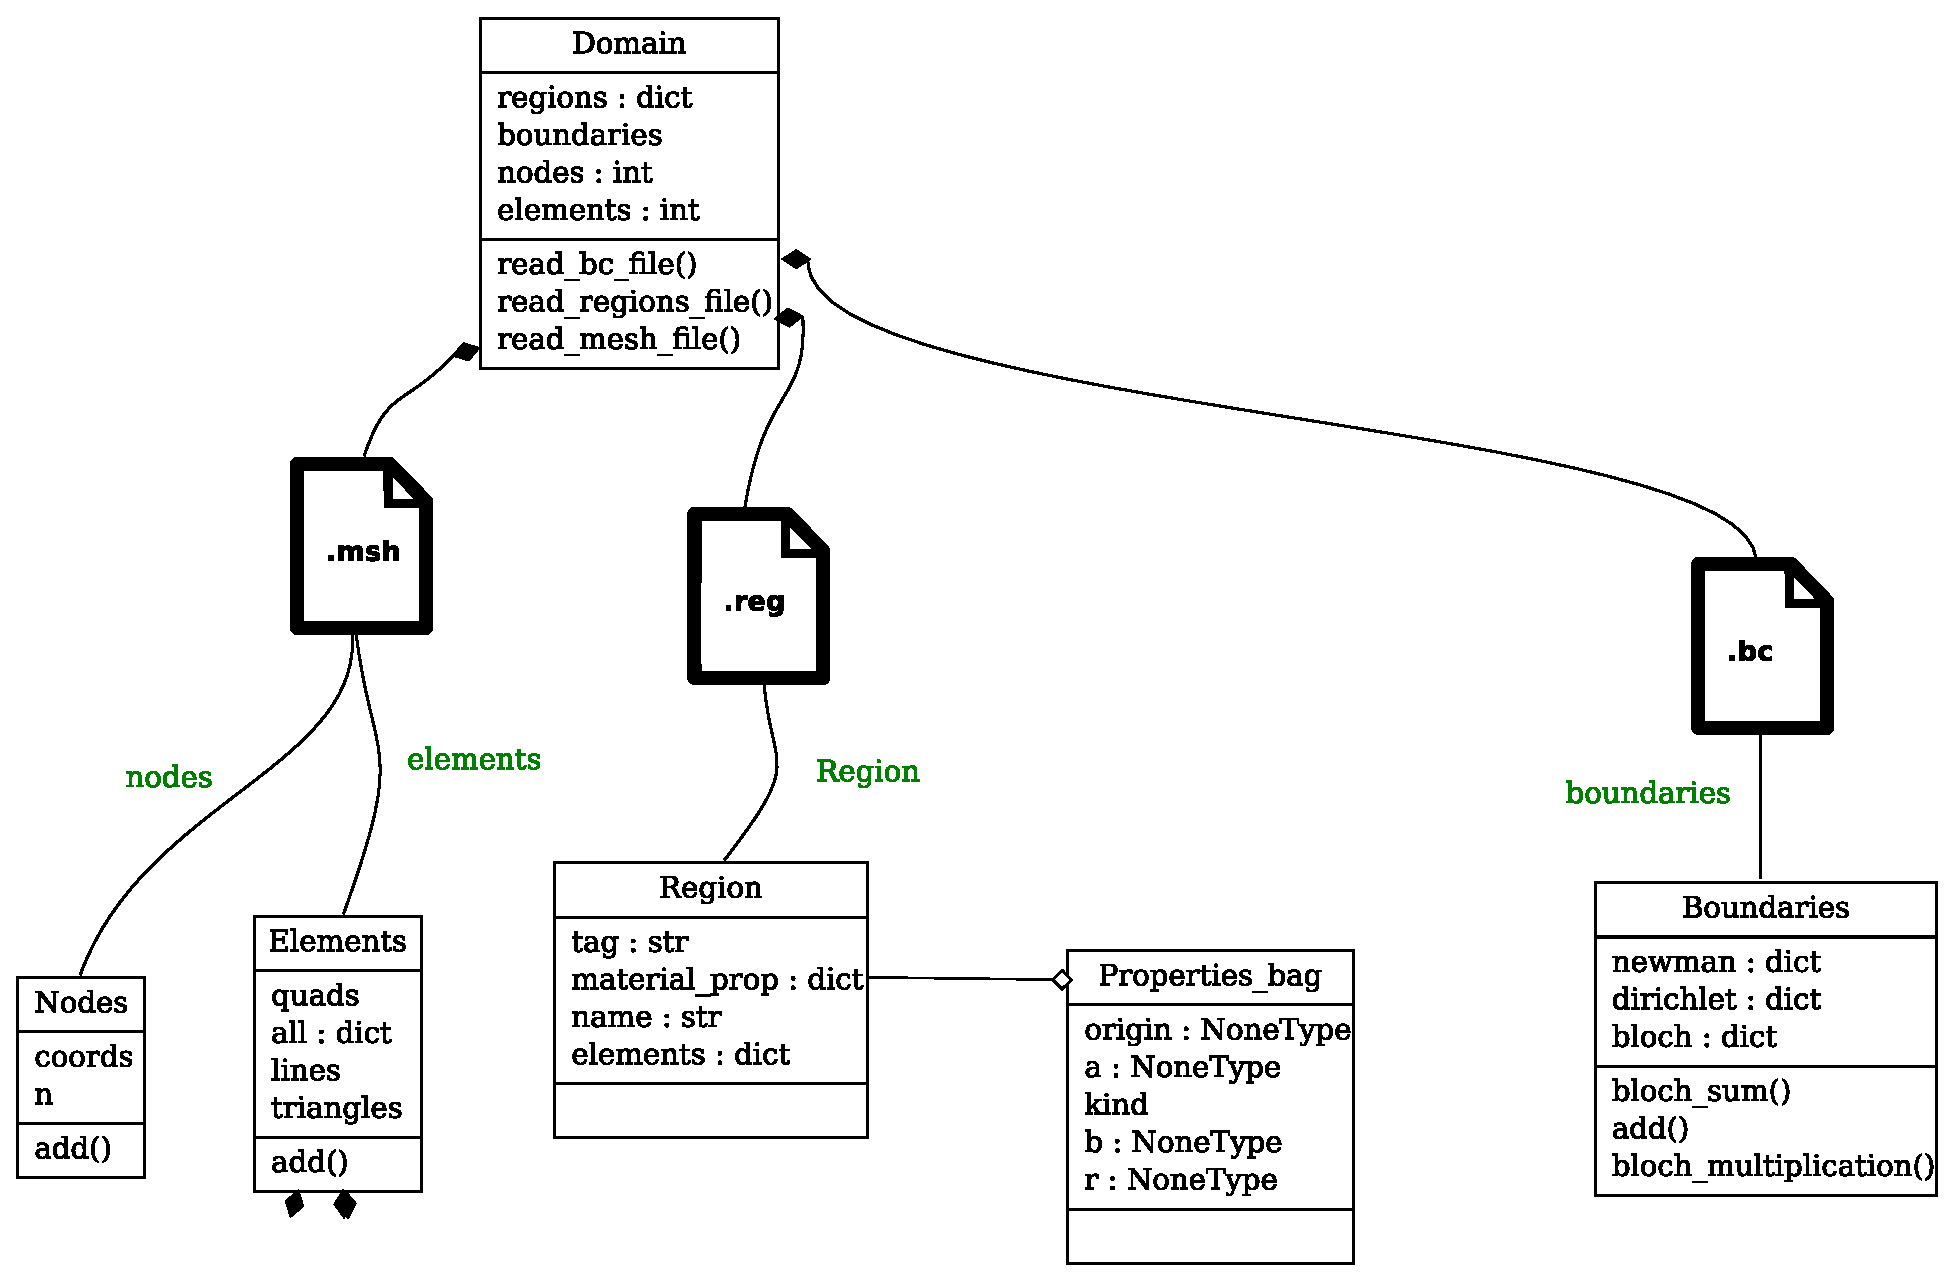
\includegraphics[scale=0.3]{classes_reduced_3.eps}
			\caption{Diagrama de clase Domain.}
			\end{figure}		
		}
		\only<6>{
			\begin{figure}
			\centering
			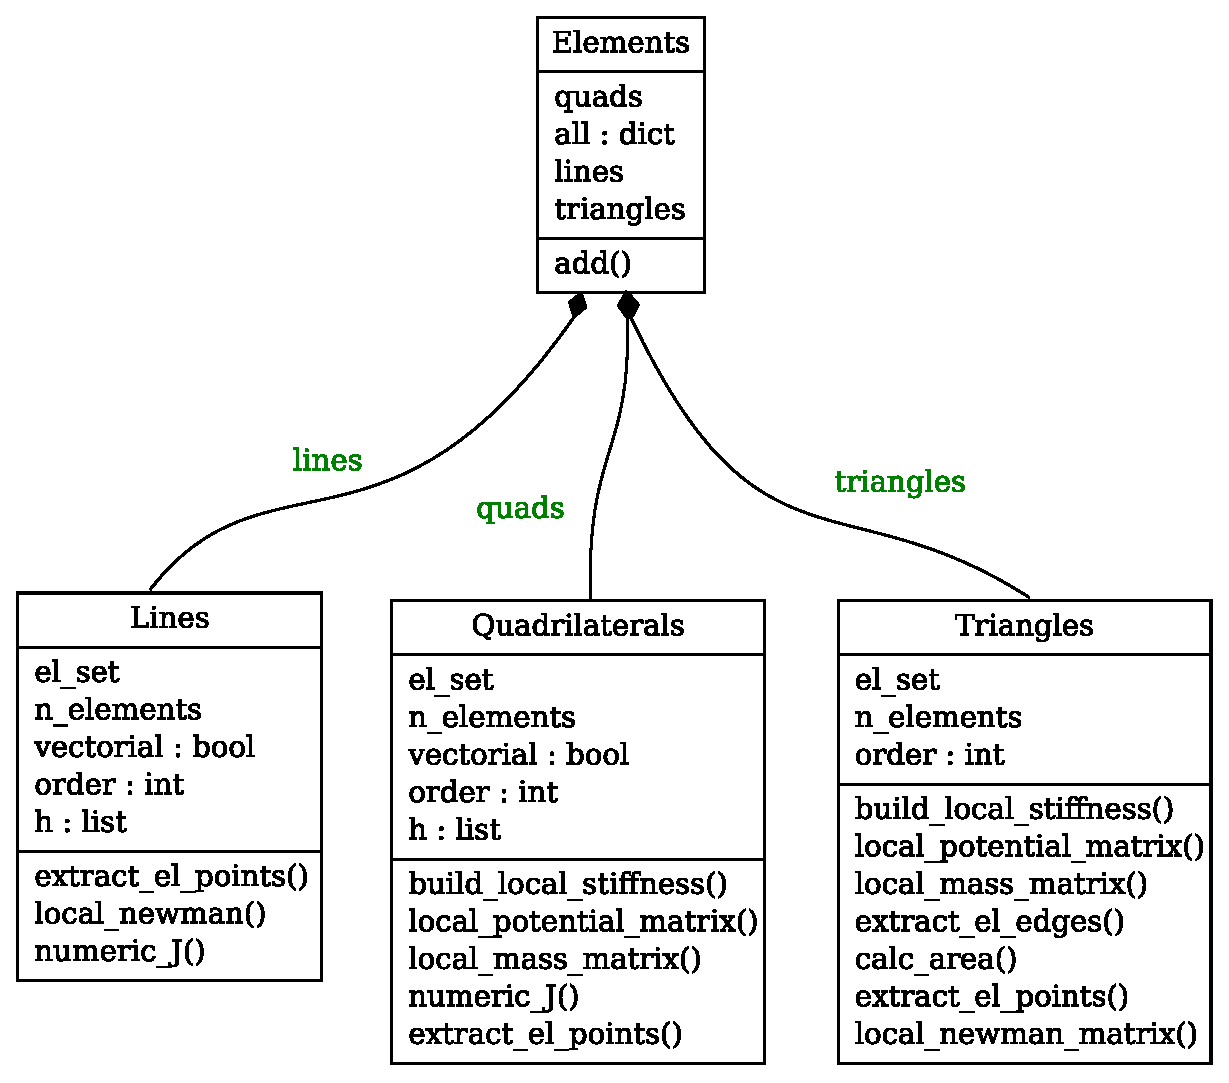
\includegraphics[scale=0.35]{classes_reduced_4.eps}
			\caption{Diagrama de clase Elements.}
			\end{figure}		
		}
	}
	\subsection{Ejemplos, y referencias}

	\begin{frame}[fragile]{¿Cómo se formula un problema en PeyeQM?}
	Se debe ejecutar un archivo que contenga las siguientes operaciones:\\
		\pause
		Importación de clases y rutinas
		\begin{python}<1>
		from Classes import Simulation
		from Interpreter import Interpreter
		from Solver import Solver
		from write import write_vtk, write_solver_input 
		from numpy import zeros
		\end{python}	
		\pause 
		Definición del nombre de archivos de entrada y parámetros de solución
		\begin{python}<2>
	filename = 'square_waveguide'
	write_solver_input(filename +'.msh',dimension = 2, bc_type = 		'Dir', \
	parameter = [], eq = 'EM', sol_type = 'Stationary',analysis_param \
	= ['y', 'y', 15, 15, 20, 20, 2], bc_filename = filename +'.bc')  
		\end{python}
	\end{frame}
	\begin{frame}[fragile]{¿Cómo se formula un problema en PeyeQM?}
	Inicialización de las clases para definir la simulación
	\begin{python}
simu = Simulation()
simu.read_solver_input(filename +'.msh')
simu.domain.read_mesh_file(filename +'.msh', True)
simu.domain.read_bc_file(simu.bc_filename)
reg_filename = simu.bc_filename.split('.bc')[0]
simu.domain.read_regions_file(reg_filename)
	\end{python}
	\pause
	Y del intérprete
	\begin{python}
inter = Interpreter()
eq = inter.build_harmonic_EM_eq(simu)
	\end{python}	
	
	\end{frame}
	\begin{frame}[fragile]{¿Cómo se formula un problema en PeyeQM?}
	Solución del sistema de ecuaciones	
	\begin{python}
	my_solver = Solver()
value, fields = my_solver.solve_spectral(simu, eq)
print len(fields), 'value', value
	\end{python}
	\pause
	Post procesamiento de la solución
	\begin{python}
quads = my_solver.substract_1(simu.domain.elements.quads.el_set)
quads = quads[:,1:]
for i in range(len(fields)):
    field3 =  zeros((simu.domain.nodes.n,3))
    field3[:,0:2] = fields[i]
    fields[i] = field3
	\end{python}
	\end{frame}
	\begin{frame}[fragile]{¿Cómo se formula un problema en PeyeQM?}
	Exportar la solución a un archivo Vtk
	\begin{python}
	write_vtk(filename +str(i)+'.vtk', 'MyTitle', 'UNSTRUCTURED_GRID' \
	 ,simu.domain.nodes.coords,\	 				
        quads, ['VECTORS', ['sol'], [fields[i]]])
\end{python}
	\end{frame}
	\begin{frame}[fragile]{Homogeneidades y cristales finitos desde PeyeQM}
		\begin{figure}
		\centering
		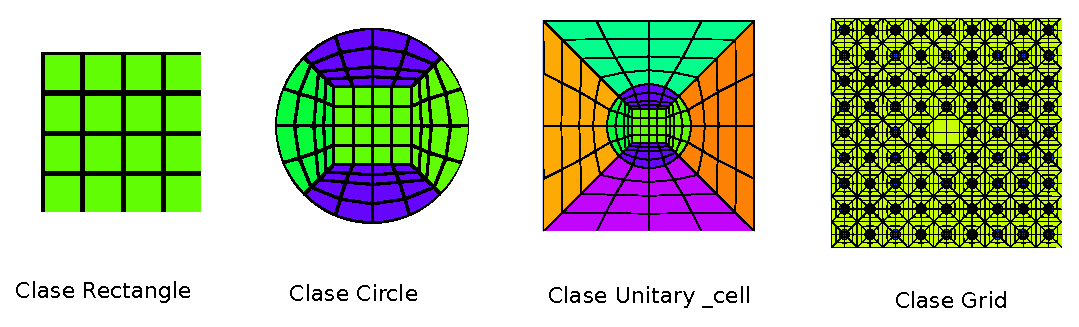
\includegraphics[scale=0.7]{gmsh_library_classes.eps}
		\end{figure}
	\end{frame}
	\begin{frame}[fragile]{Homogeneidades y cristales finitos desde PeyeQM}
	\begin{columns}
		\column{0.5\textwidth}
		\tiny
			\begin{python}
	from gmsh_library import *
	point = Point(0,0,0)

a = 1
phys_tag_outside = 30
phys_tag_inside = 31

frame = \
Unitary_cell(0, point, a, a, \
transfinite = (2,1), \
phys_tag = phys_tag_outside)

circle_center = \
Point(frame.points[-1].id_tag, a/2.,a/2.)

frame.add_circular_inclussion(1,\
circle_center,0.2, \
phys_tag = phys_tag_inside)

lumpy.object_diagram()
for s in frame.surfaces[5:]:
    print s
f = open('unit_cell_1-02_two_reg.geo','w')
f.write(frame.__str__())
f.close
			\end{python}
		\column{0.5\textwidth}
			\begin{figure}
			\centering
			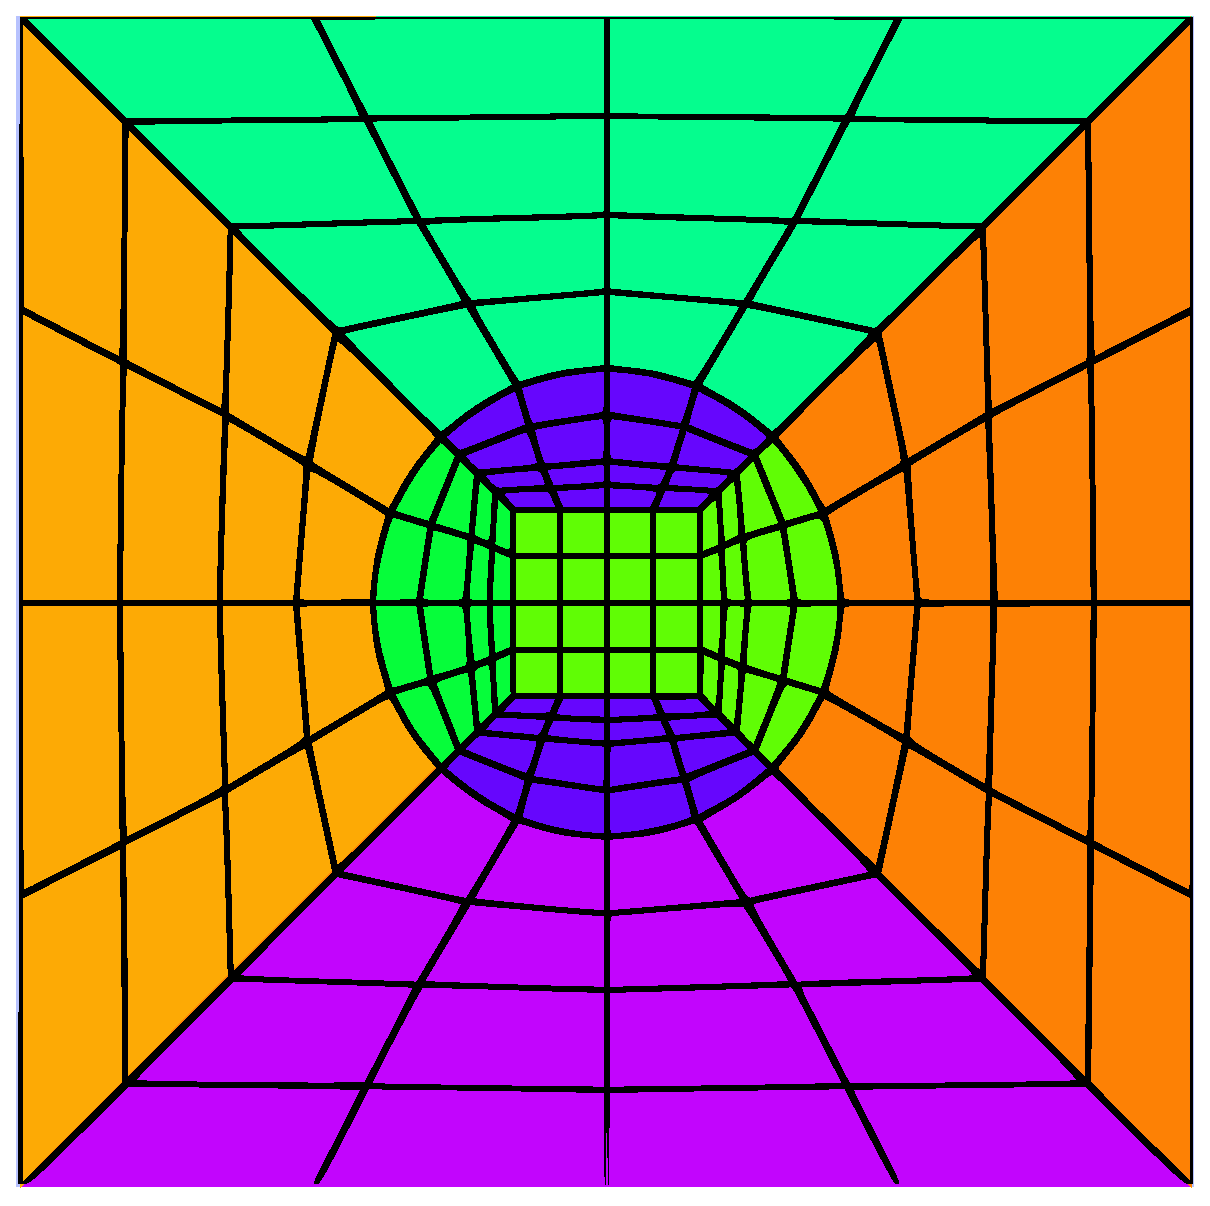
\includegraphics[scale=0.2]{unit_cell_pretty.eps}
			\end{figure}
		\end{columns}
	\end{frame}
	\begin{frame}[fragile]
		\begin{columns}
			\column{0.5 \textwidth}		
			\tiny
			\begin{python}
			from gmsh_library import * 
blc = Point(0,0,0) #Bottom left corner
a = 1 # unit cell width
cc = Point(0, a/2.,a/2.) # circle center

phys_tag_outside = 30
phys_tag_inside = 31

pt = [phys_tag_outside, phys_tag_inside] 

sketch =
 [['1','1','1','1','1','1','1','1','1'],
  ['1','1','1','1','1','1','1','1','1'],
  ['1','1','1','1','1','1','1','1','1'],
  ['1','1','1','1','1','1','1','1','1'],
  ['1','1','1','1','0','1','1','1','1'],
  ['1','1','1','1','1','1','1','1','1'],
  ['1','1','1','1','1','1','1','1','1'],
  ['1','1','1','1','1','1','1','1','1'],
  ['1','1','1','1','1','1','1','1','1']]
  
c = Properties_bag('circle', \
		 origin = cc, r = 0.2)
e = Properties_bag('empty')
d = {'1': c,'0':e}

domain = Grid(blc, a, sketch, d,\
 phys_tags = pt, transfinite = (2,1))
domain.define_boundary()

f = open('finite_lattice_point_defect.geo','w')
f.write(domain.__str__())
f.close
			\end{python}
			\column{0.5\textwidth}
			\begin{figure}
			\centering
			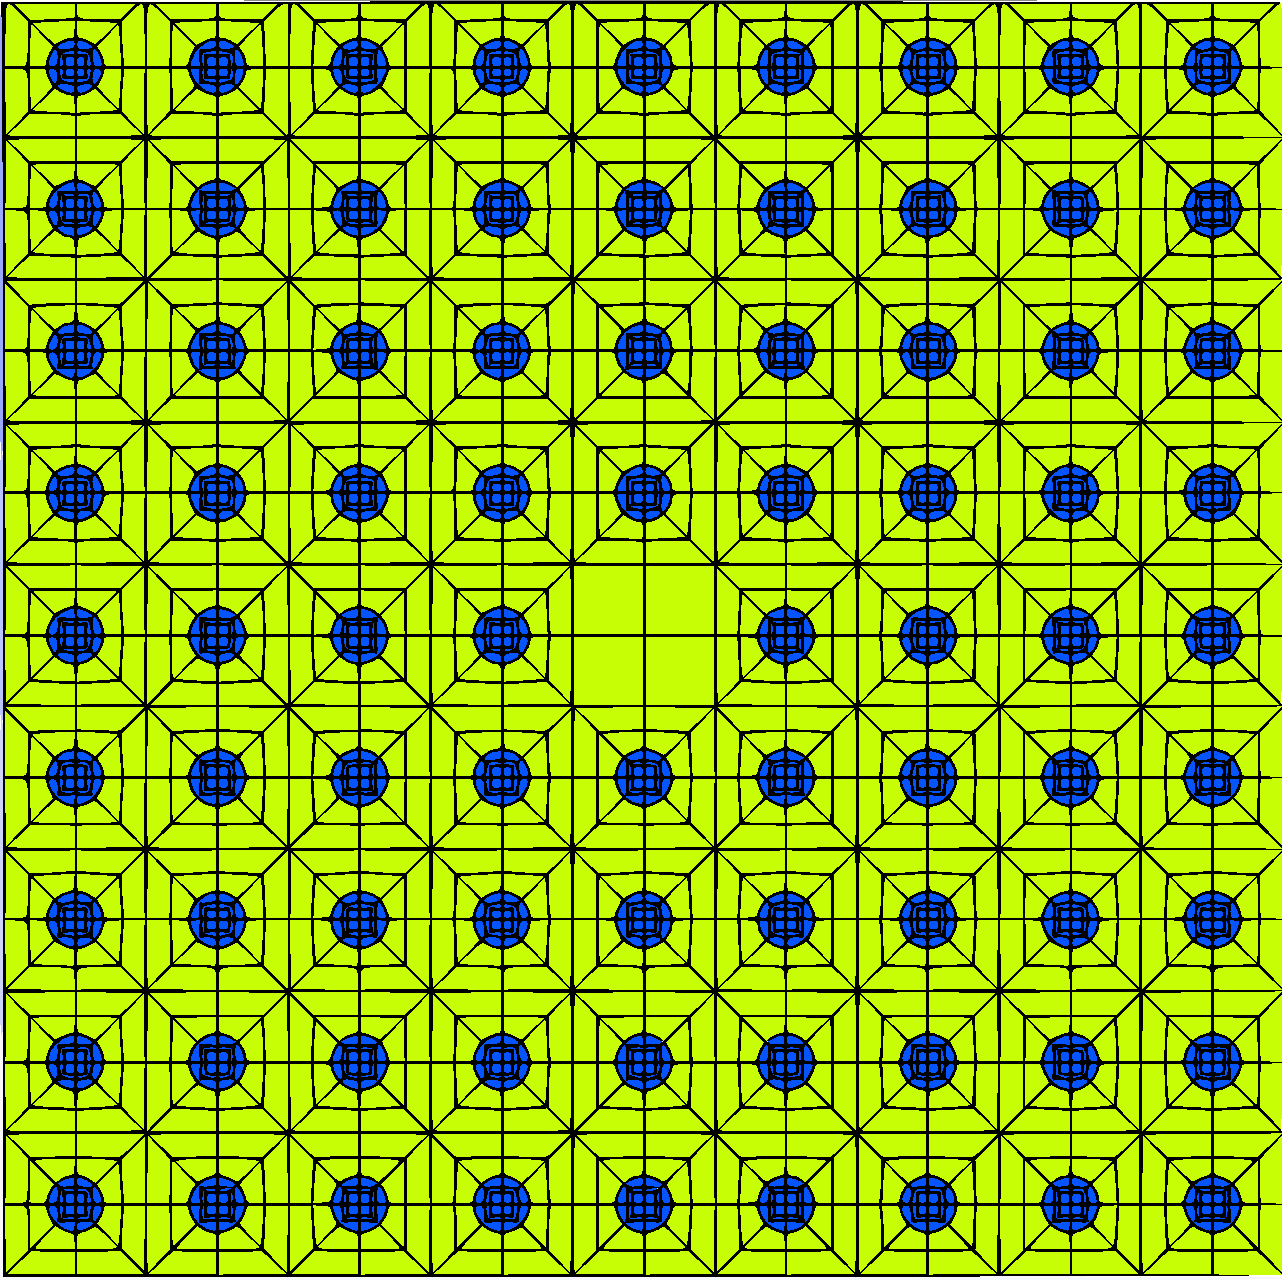
\includegraphics[scale=0.2]{lattice_point_deffect.pdf}
			\end{figure}
		\end{columns}
	\end{frame}
\section{Resultados}
%	\subsection{Pruebas de problemas electrostáticos}
%	\begin{frame}{Pruebas de problemas electrostáticos}
%	\begin{figure}
%	\centering
%	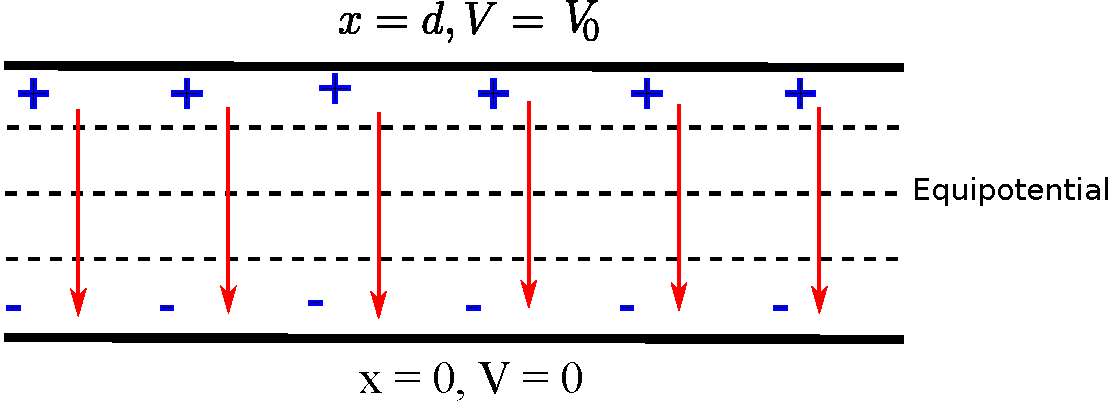
\includegraphics[scale=0.5]{parallel_plate_capacitor.pdf}
%	\caption{Capacitor de placas paralelas.}
%	\end{figure}
%	\begin{figure}
%	\centering
%	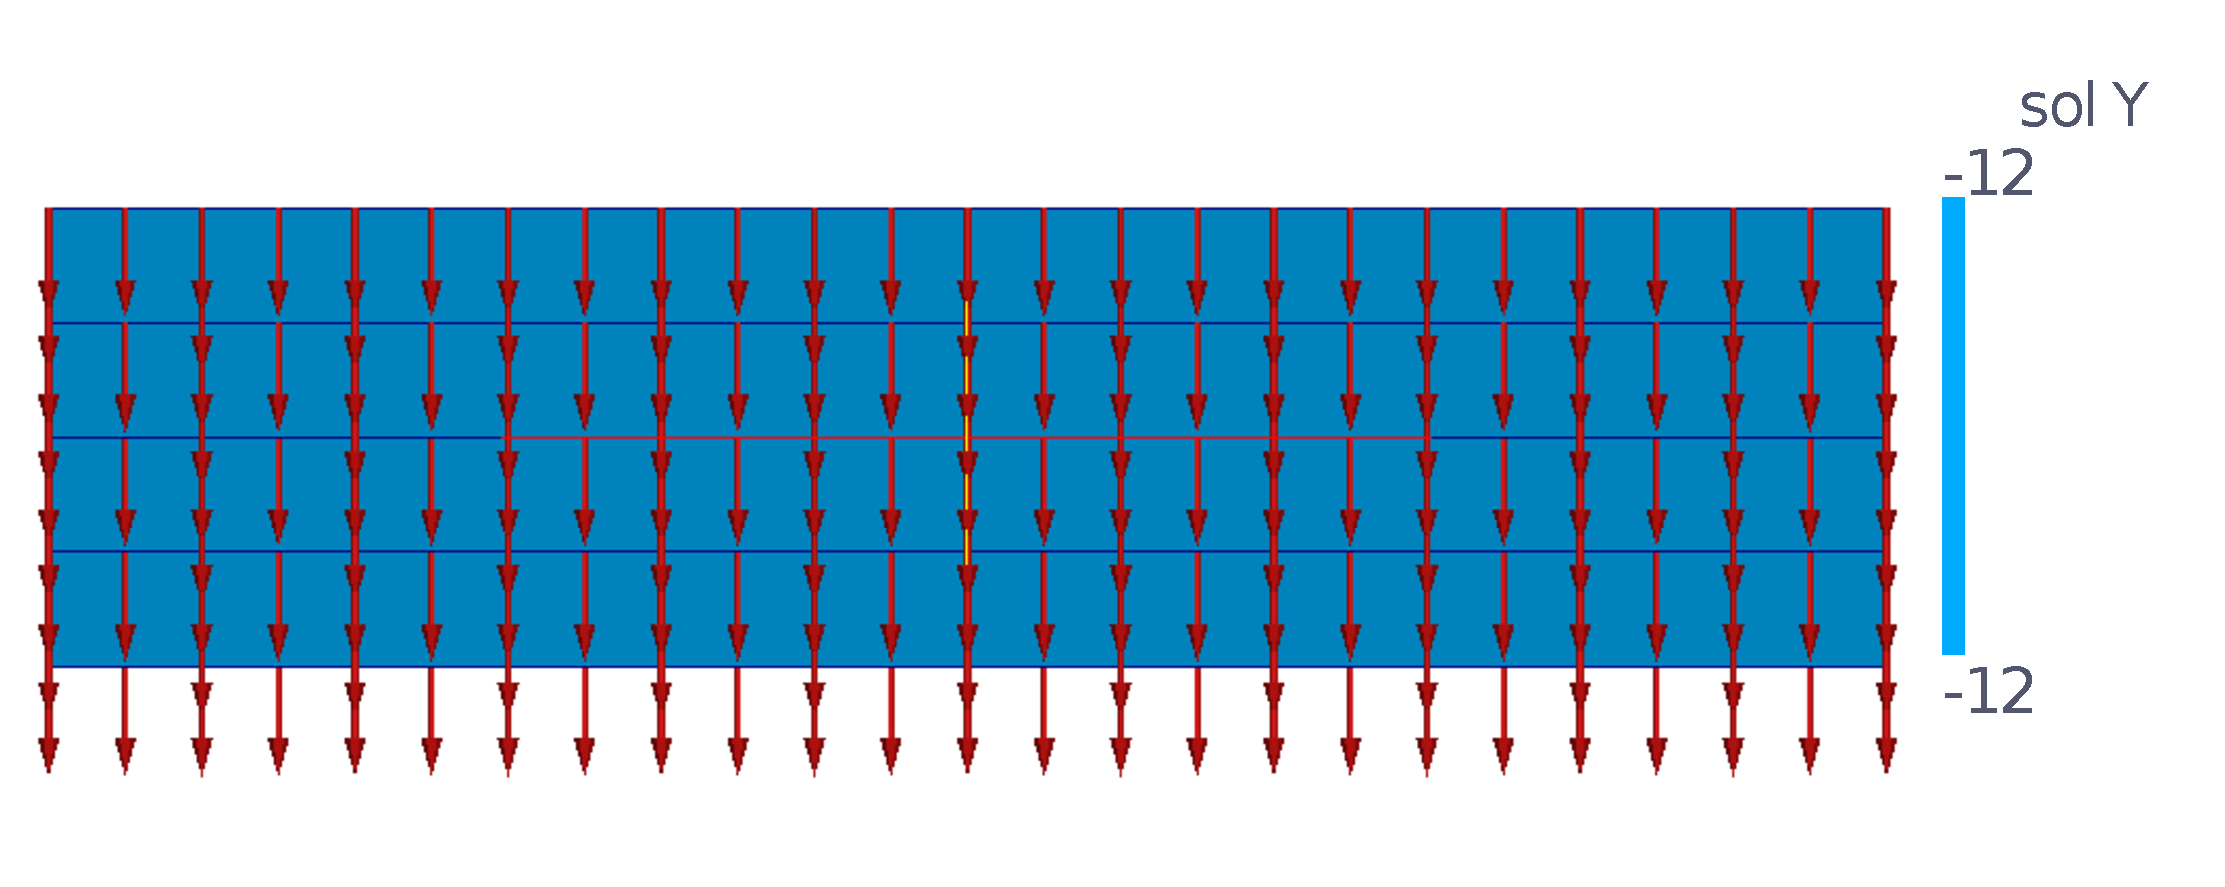
\includegraphics[scale=0.3]{capacitor.pdf}
%	\caption{Simulación de campo en un capacitor de placas paralelas.}
%	\end{figure}	
%	\end{frame}
	\subsection{Pruebas de problemas electrostáticos}
	
	\begin{frame}{Pruebas de problemas electrostáticos}
		\begin{figure}
		\centering
		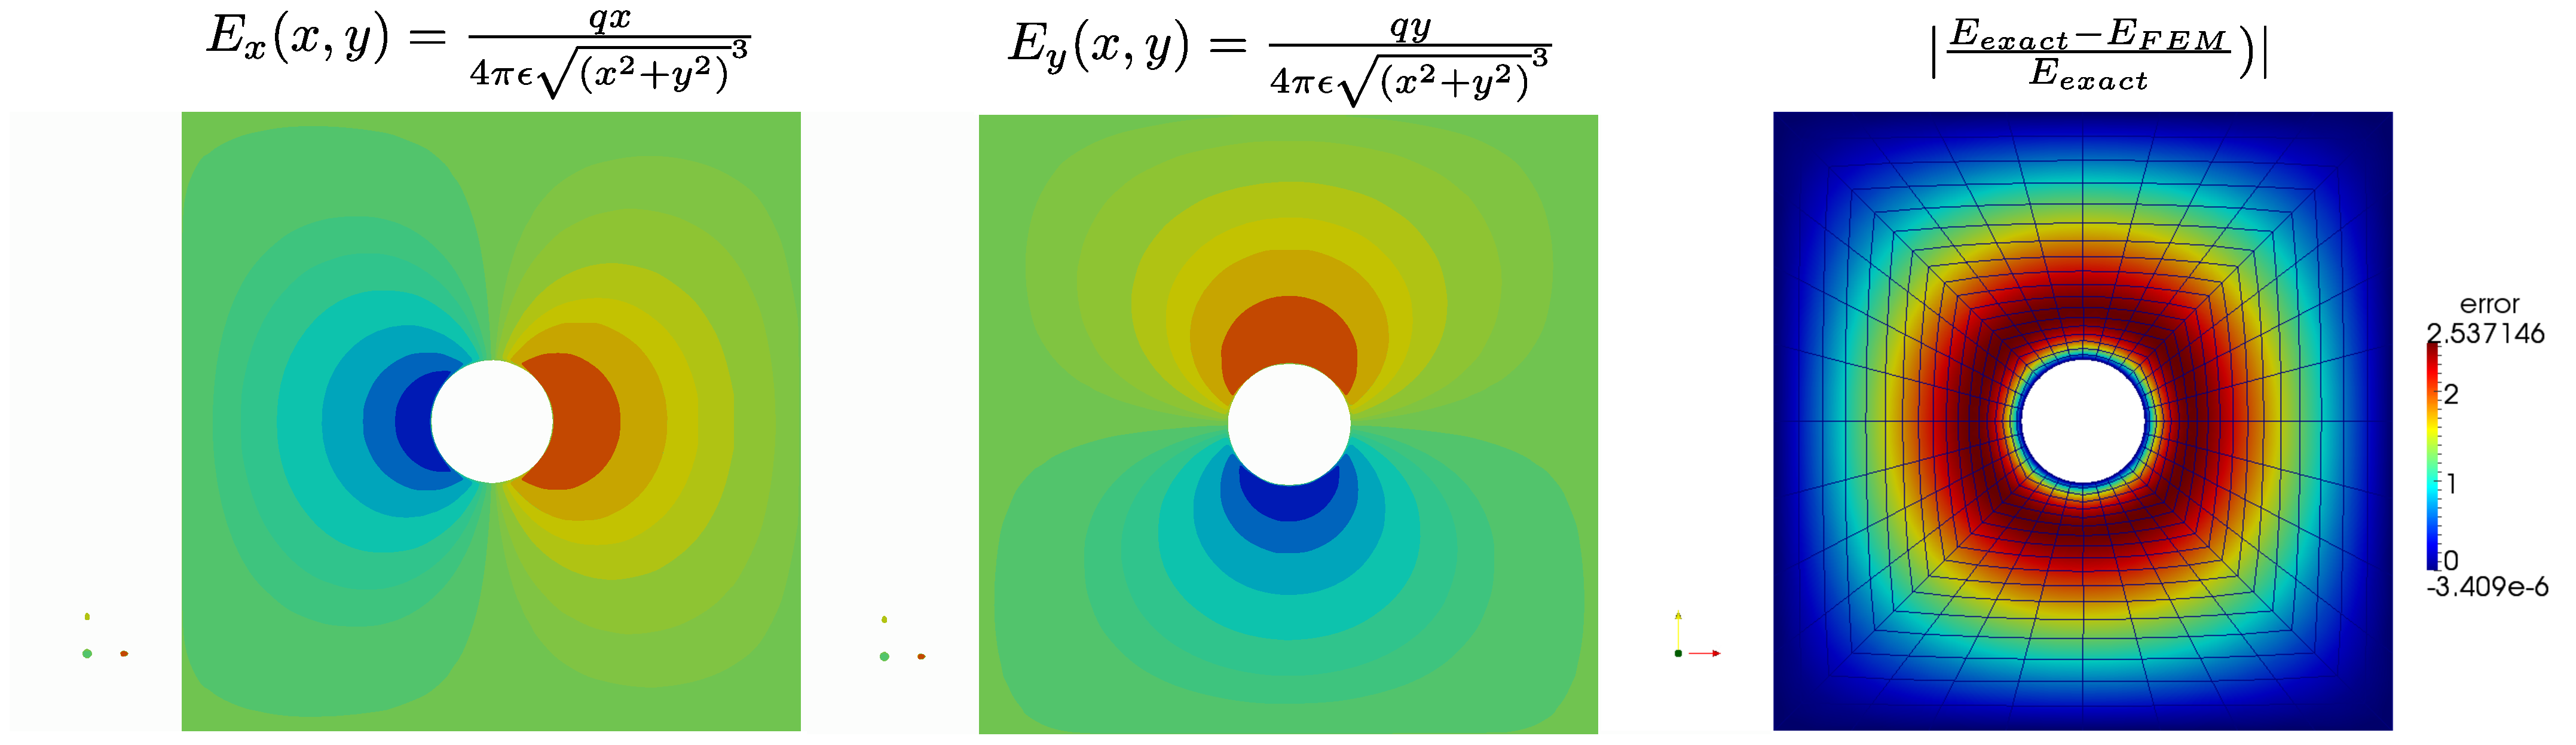
\includegraphics[scale=0.15]{charged_cylinder_inside_rectangle.eps}
		\caption{Simulación de el campo eléctrico debido a un cilindro cargado.}
		\end{figure}
	\end{frame}
	\begin{frame}{Pruebas de problemas electrostáticos}
		\begin{figure}
		\centering
		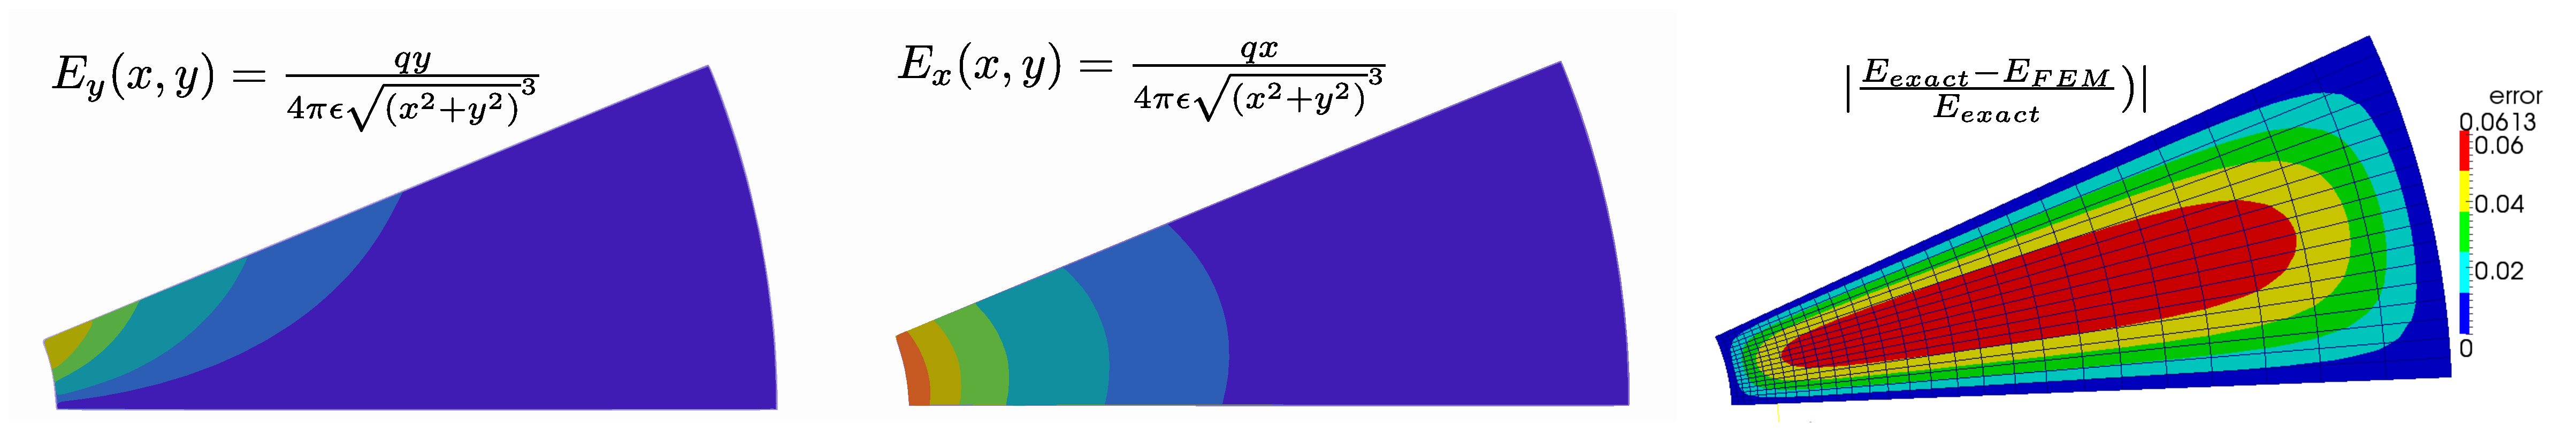
\includegraphics[scale=0.15]{Eight_of_cylinder.eps}
		\caption{Segmento de un octavo de la simulación del campo eléctrico debidos a un cilindro cargado.}
		\end{figure}
	\end{frame}
	\begin{frame}{Pruebas de problemas electrostáticos}
		\begin{figure}
		\centering
		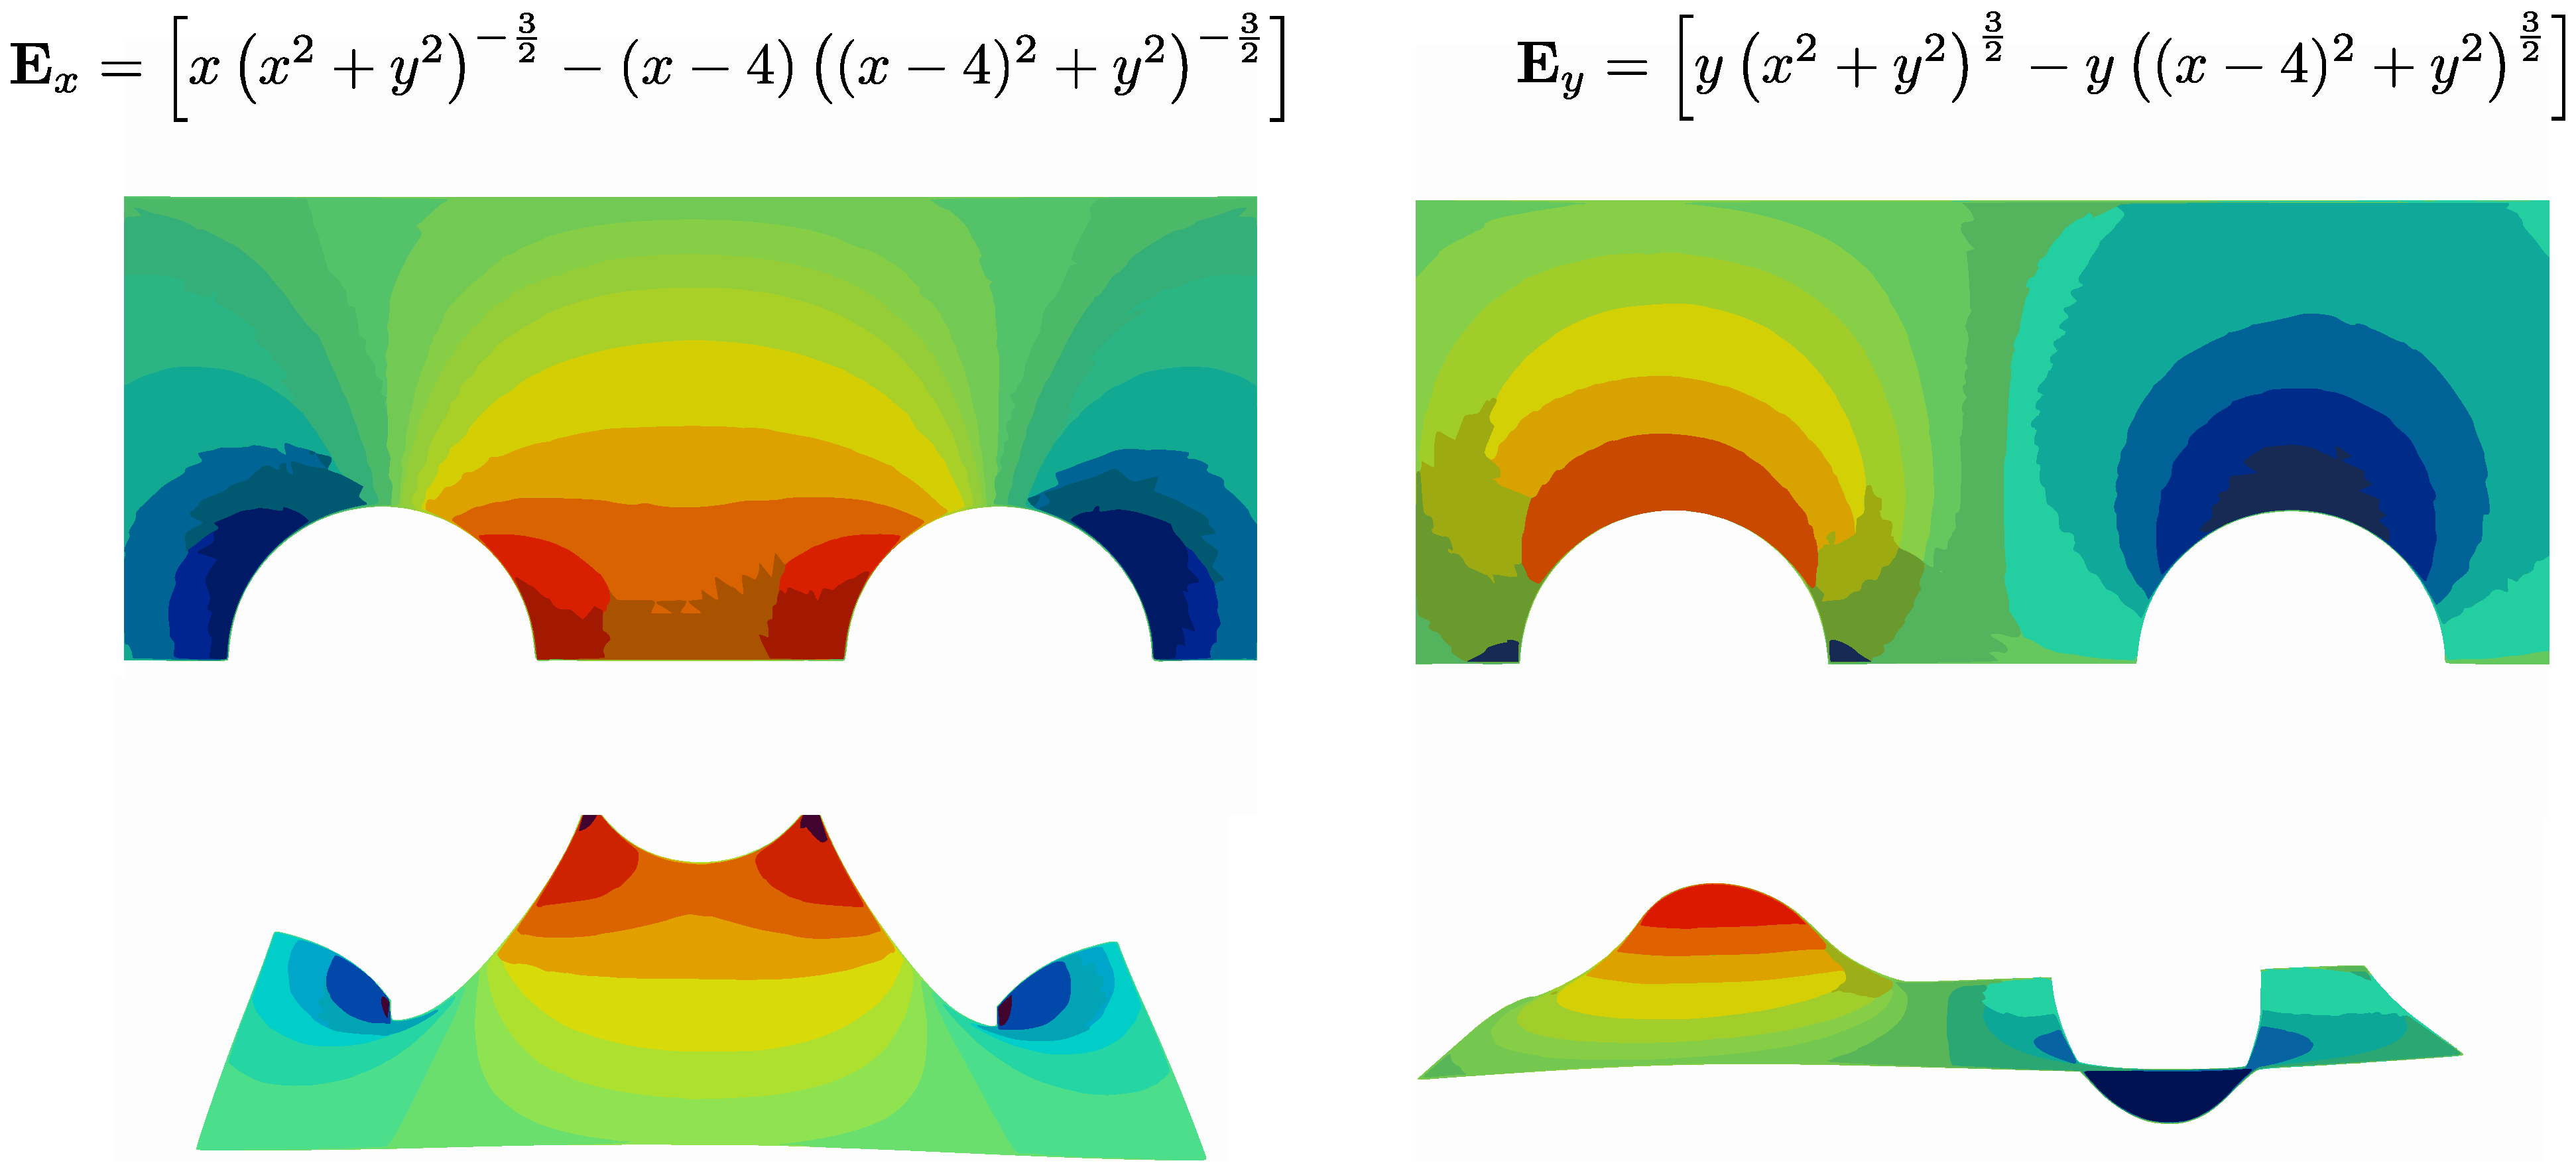
\includegraphics[scale=0.18]{two_cylinders.eps}
		\caption{Componentes del campo eléctrico luego de simular el efecto de dos cilindros cargados.}
		\end{figure}
	\end{frame}
	\begin{frame}{Pruebas de problemas electrostáticos}
		\begin{figure}
		\centering
		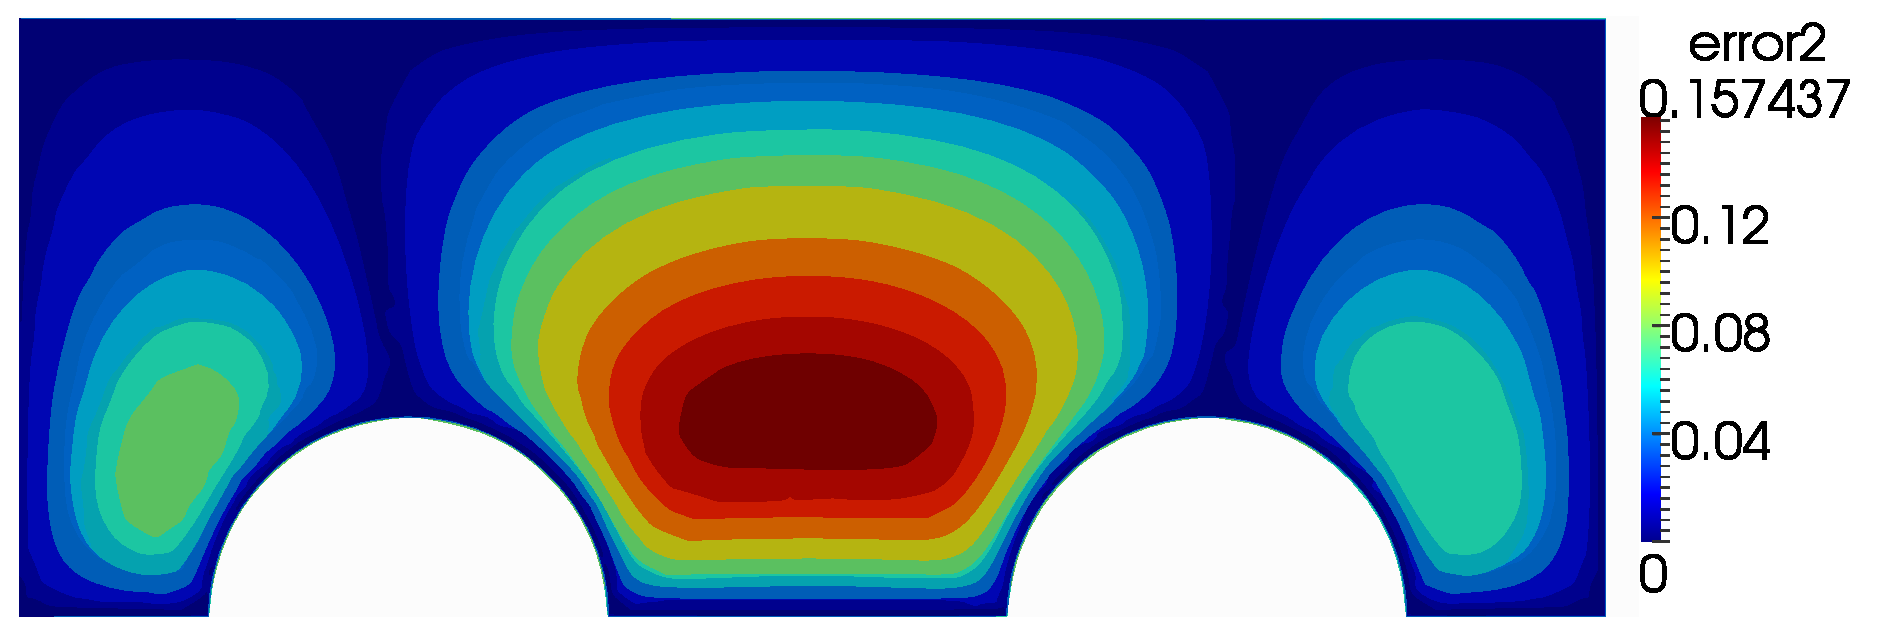
\includegraphics[scale=0.4]{two_cylinders_error.eps}
		\caption{Cálculo del error para el problema de dos cilindros cargados.}
		\end{figure}
	\end{frame}
	\subsection{Pruebas de problemas armónicos}
	\begin{frame}{Pruebas de problemas armónicos}
		\begin{figure}
		\centering
		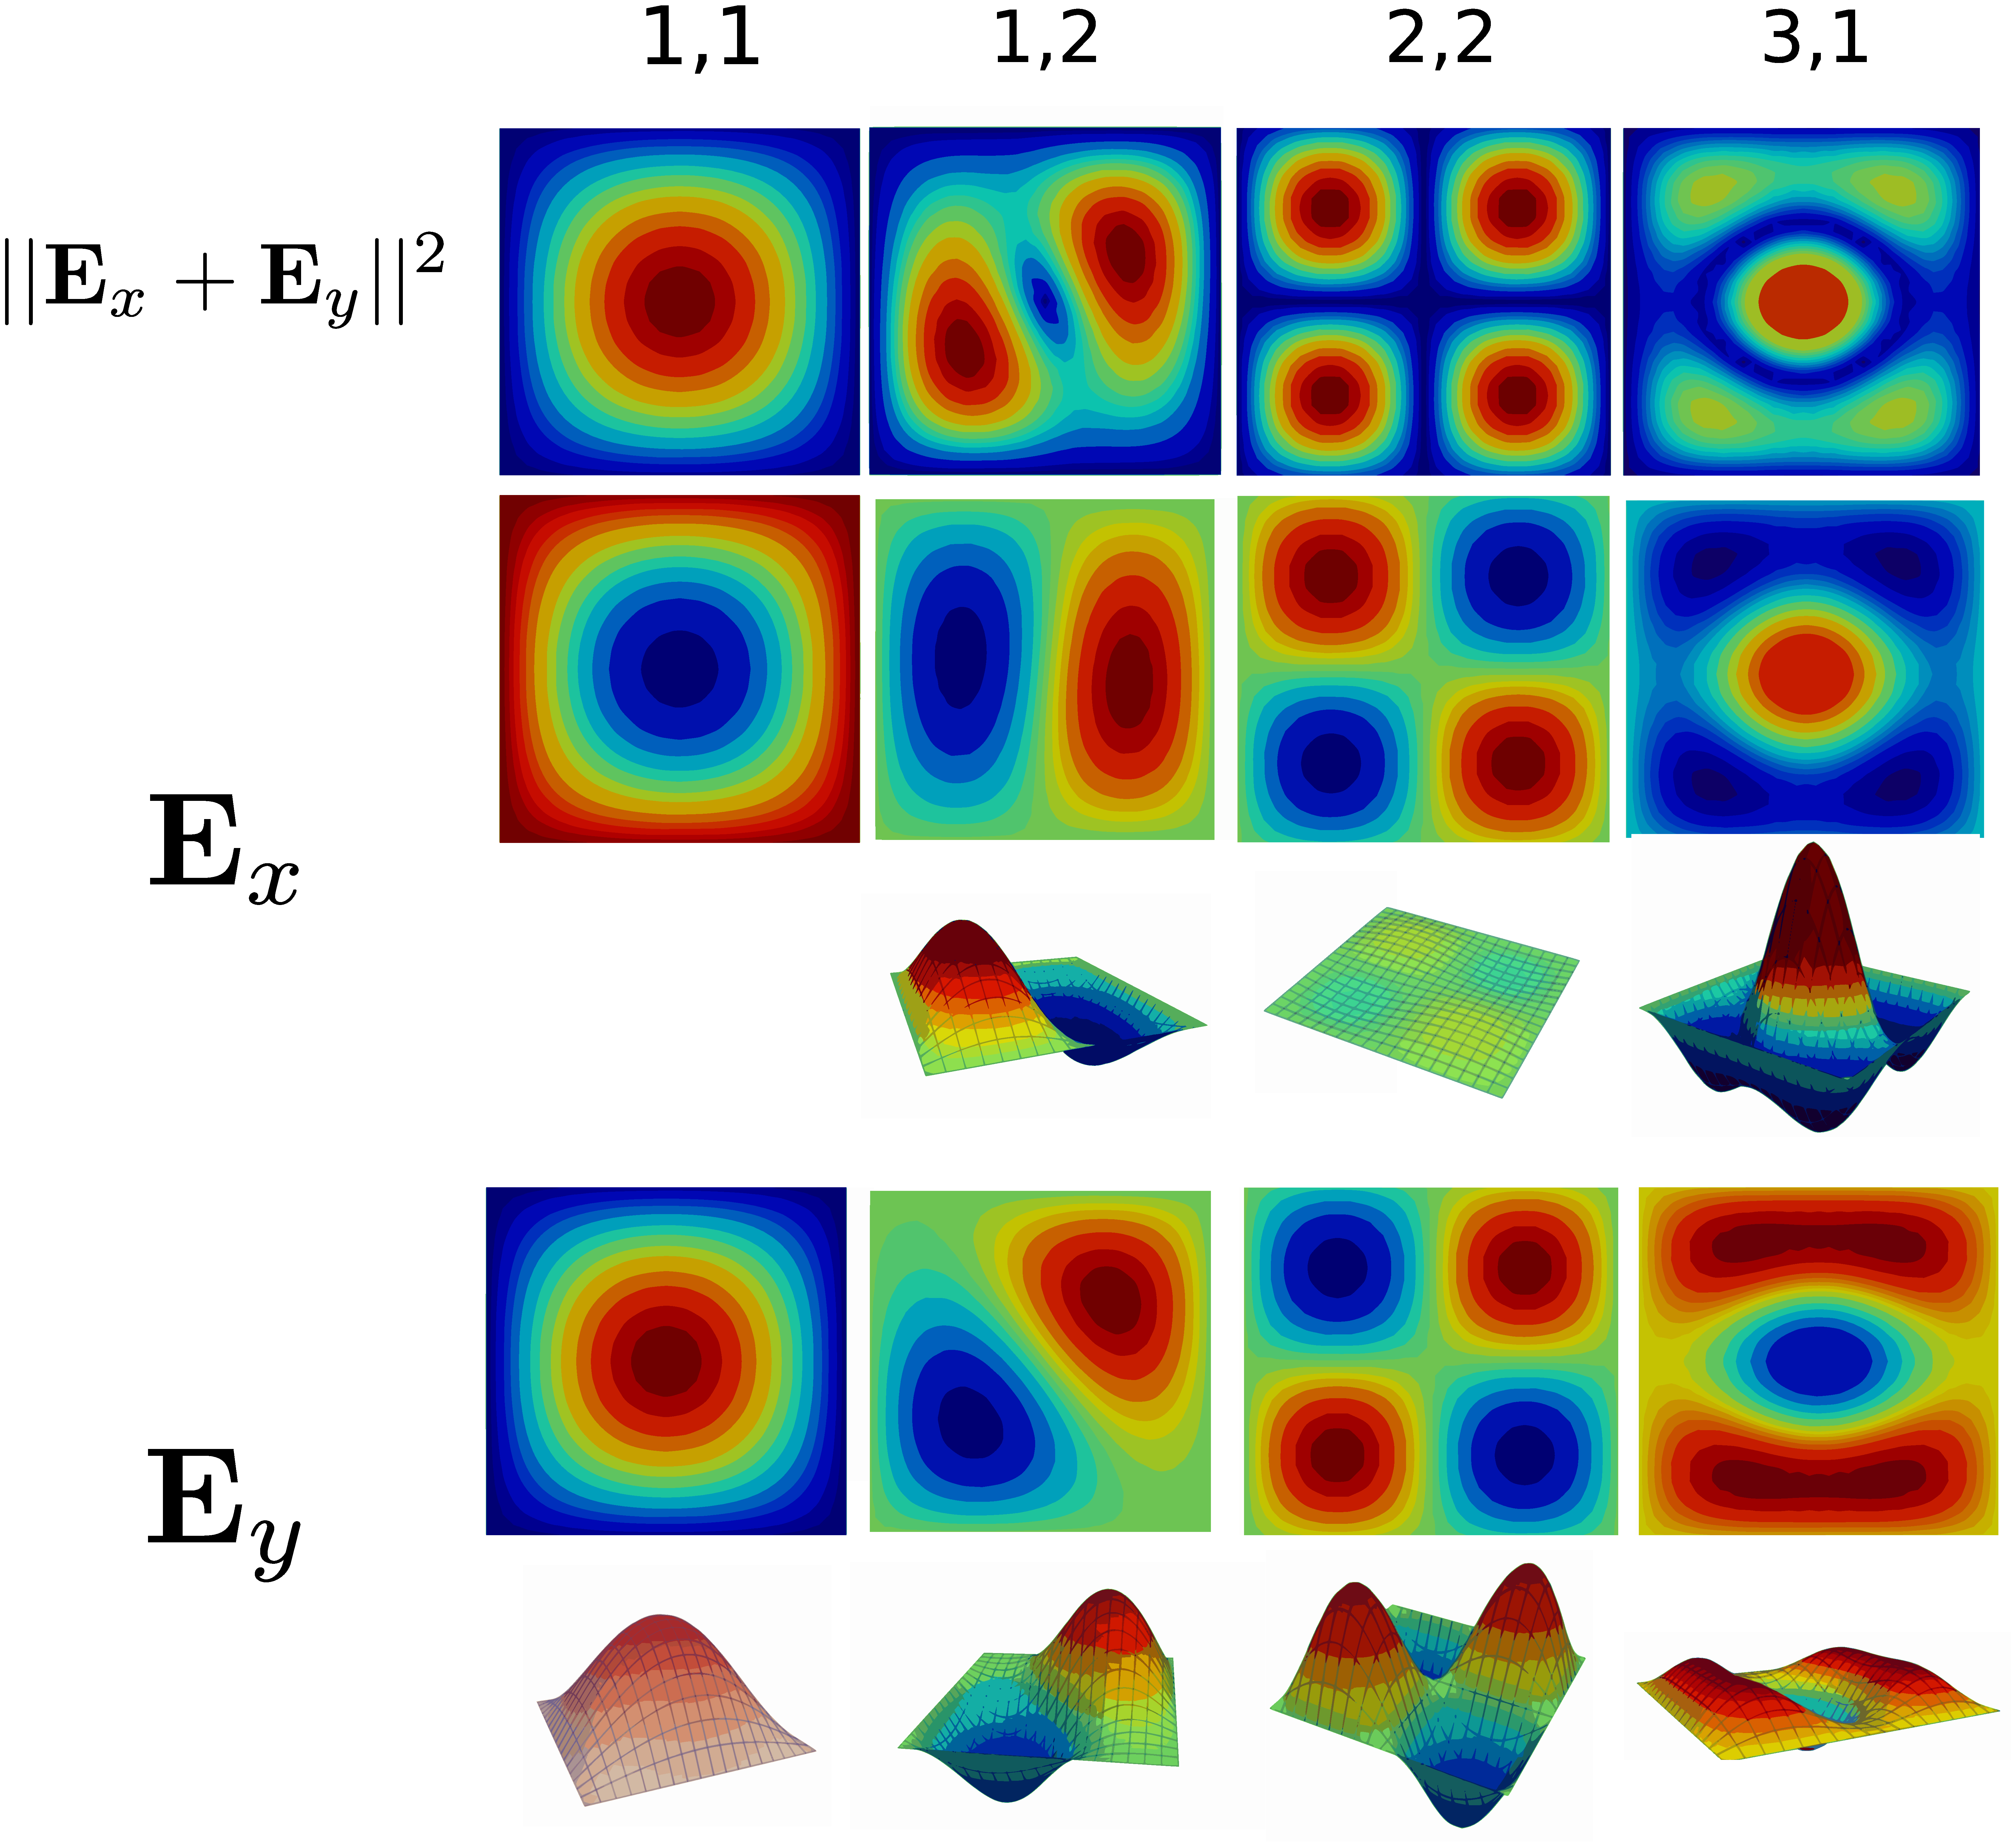
\includegraphics[scale=0.07]{square_waveguide.eps}
		\caption{Resultados para tres modos distintos de la simulación de guías de onda cuadrada $a=b=2$.}
		\end{figure}
	\end{frame}
	\begin{frame}{Pruebas de problemas armónicos}
		\begin{figure}
		\centering
		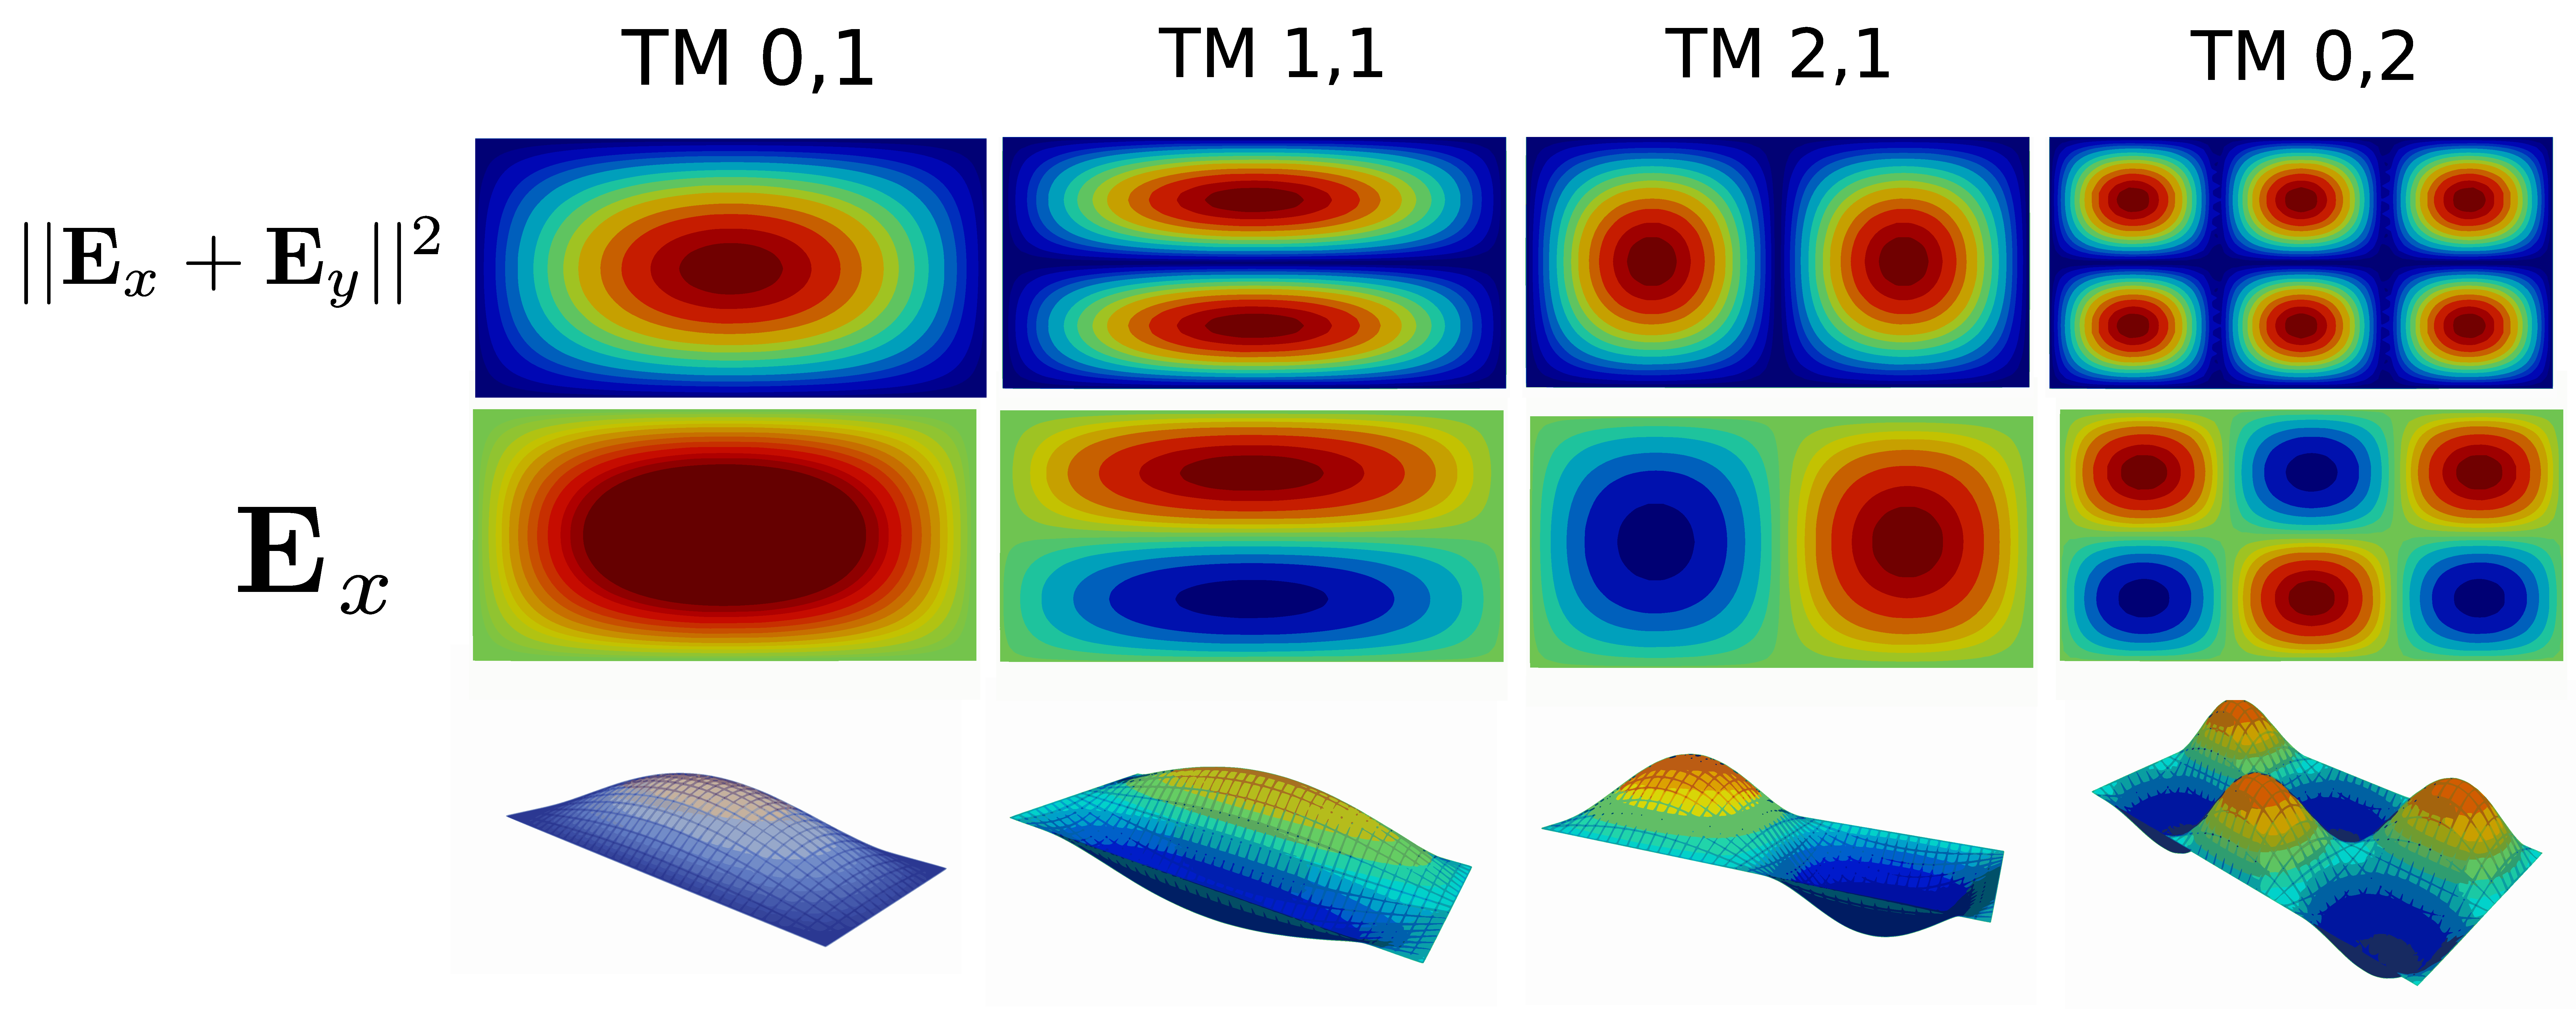
\includegraphics[scale=0.06]{rectangular_waveguide.pdf}
		\caption{Resultados de simulación para guías de onda rectangulares con lados $a=4$ y $b=2$.}
		\label{fig:rectangular_waveguide}
		\end{figure}
	\end{frame}
	\begin{frame}{Pruebas de problemas armónicos}
		\begin{center}
		\begin{tabular}{|c|c|c|c|c|}
		\hline
		\multicolumn{5}{|c|}{Comparación de $\omega^2$ para guías de onda cuadradas} \\
		\hline 
		m,n & 1,1 & 1,2 & 2,2 & 3,1 \\ 
		\hline 
		FEM & 4.93480857 & 12.33721117 & 19.73961759 & 24.6763011 \\ 
		\hline 
		Analítico & 4.93480220 & 12.33700550 & 19.73920880 & 24.67401100 \\ 
		\hline 
		\end{tabular} 
		\end{center}
		\begin{center}
	\begin{tabular}{|c|c|c|c|c|}
	\hline
	\multicolumn{5}{|c|}{Comparación de $\omega^2$ para guías rectangulares de lado $a =2b$} \\
	\hline 
	m,n & 1,1 & 2,1 & 3,1 & 1,2 \\ 
	\hline 
	FEM     & 3.08425459 & 4.93480795 & 8.0190859 & 12.33717191 \\ 
	\hline 
	Analítico & 3.08425137 & 4.93480220 & 8.0190535 & 12.33700550 \\ 
	\hline 
	\end{tabular} 
	\end{center}
	\end{frame}
	\begin{frame}{Prueba de problemas armónicos}
	\begin{figure}
\centering
\includegraphics[scale=0.07]{circular_waveguide.eps}
%\caption{Resultados de tres modos para la simulación de cavidades resonantes circulares con radio $a=2$.}
\small
\begin{center}
\begin{tabular}{|c|c|c|c|c|}
\hline
\multicolumn{5}{|c|}{Comparación de $\frac{\omega}{a}$ para guía de onda circular.} \\
\hline 
m,n & 0,1 & 1,1 & 2,1 & 0,2 \\ 
\hline 
FEM     & 2.40482634 & 3.83171343 & 5.13564189 & 5.52012378 \\ 
\hline 
Analítico & 2.40482555 & 3.83170597 & 5.13562230 & 5.52007811 \\ 
\hline 
\end{tabular} 
\end{center}
\end{figure}	
	\end{frame}
	\begin{frame}{Prueba de problemas armónicos}
	\begin{figure}
\centering
\includegraphics[scale=0.07]{hexagonal_waveguide.pdf}
\end{figure}
\small
\begin{center}
\begin{tabular}{|c|c|c|c|c|}
\hline
\multicolumn{5}{|c|}{Primeras 4 frecuencias $\omega^2$ de una cavidad resonante hexagonal.} \\
\hline 
m,n & 0,1 & 1,1 & 2,1 & 0,2 \\ 
\hline 
FEM     & 5.34990939 & 8.51630317 & 11.39340788 & 12.2461672 \\ 
\hline 
\end{tabular} 
\label{tab:hex_wav_comparison}
\end{center}
	\end{frame}
	\begin{frame}{Pruebas de problemas armónicos}
		\begin{figure}
		\centering
		\includegraphics[scale=0.07]{elliptical_waveguide.eps}
		\caption{Modos en cavidad resonante elíptica con eje menor  $a=2$ y eje mayor $b=3$.}
		\end{figure}	
		\begin{center}
		\begin{tabular}{|c|c|c|c|c|}
		\hline
		\multicolumn{5}{|c|}{Primeras cuatro frecuencias $\omega$} 		\\
		\hline 
		FEM & 2.0195 & 2.4149 & 2.6627 & 2.9457 \\ 
		\hline 
		\end{tabular} 
		\end{center}	
	\end{frame}
	\begin{frame}{Pruebas de problemas armónicos}
		\begin{figure}
		\centering
		\includegraphics[scale=0.11]{isoespectral.eps}
		\caption{Modos de dos cavidades iso-espectrales tomadas de \cite{Chapman1995}.}
		\label{fig:isoespectral_waveguide}
		\end{figure}
		\small
		\begin{center}
		\begin{tabular}{|c|c|c|c|c|}
		\hline
		\multicolumn{5}{|c|}{Comparación de $\omega^2$} \\
		\hline 
Shape 1  & 6.38705867 & 7.65676809 & 9.11294713 & 10.23292227 \\ 
		\hline 
Shape 2 & 6.3850403 & 7.65926504 & 9.11794073 & 10.23394057 \\ 
		\hline 
		\end{tabular}
		\end{center}
	\end{frame}
	\begin{frame}{Pruebas de cristales finitos}
		\begin{figure}
		\centering
		\includegraphics[scale=0.05]{finite_lattice.eps}
		%\caption{A lattice of dielectric rods embedded in a domain causes peaks of field magnitude in the places with higher dielectric constant.}
		\end{figure}
	\end{frame}
	\begin{frame}{Pruebas de cristales finitos}
	\small
	\begin{center}
		\begin{tabular}{|c|c|c|c|c|}
		\hline
		\multicolumn{5}{|c|}{Comparación de $\omega$ para una red finita.} \\
\hline 
m,n & 1,1 & 1,2 & 2,2 & 3,1 \\ 
\hline 
varillas dieléctricas & 0.77475487 & 1.19190369 & 1.46064033 & 1.58328716 \\ 
\hline 
Aire  & 1.11074305 & 1.75637223 & 2.22176045 & 2.48458998 \\ 
\hline 
\end{tabular}

\end{center}
	\end{frame}
	\subsection{Pruebas de cristales infinitos}
	\begin{frame}{Pruebas de cristales infinitos}
	\only<1>{
	\begin{figure}
\centering
\includegraphics[scale=0.2]{reduced_brillouin_zone.pdf}
\caption{Ilustración de la zona de Brillouin y el contorno que se usa para los gráficos de bandas.}
\end{figure}
	}
	\only<2>{
	\begin{figure}
	\centering
	\includegraphics[scale=0.5]{square_lattice_ra01.pdf}
	\end{figure}
	}
	\only<3>{
	\begin{figure}
	\centering
	\includegraphics[scale=0.5]{square_lattice_ra02.pdf}
	\end{figure}
	}
	\only<4>{
	\begin{figure}
	\centering
	\includegraphics[scale=0.5]{square_lattice_ra04.pdf}
	\end{figure}
	}
	\end{frame}
\section{Conclusiones y trabajo futuro}	
	\subsection{Trabajo futuro}
	\begin{frame}
		\frametitle{Trabajo futuro}
		¿Qué vale la pena explorar en trabajos futuros?		
		\begin{itemize}
		\pause
		\item Elementos triangulares vectoriales y de segundo orden.
		\pause		
		\item  Elementos cuadriláteros lineales y escalares.
		\pause
		\item Añadir soporte para condiciones de frontera infinitas de alguno de estos tipos:
		\begin{itemize}
			\pause
			\item  Perfectly Matched Layers PML\cite{Jin2010}. 
			\pause
			\item Uso de condiciones de frontera de Robin cuando la impedancia intrínseca es conocida.
			\pause
			\item Mapeo  de la región no acotada a una geometría conocida (e.g con mapeo conformal). \pause
		\item Formulación híbrida de  FEM y Boundary Elements(BEM) como la implementada por Nicol\'as Guar\'in en \cite{Guarin2012}.
		\pause
		\item Elementos Infinitos, caso especial de los elementos finitos con un comportamiento de decaimiento (\cite{Zienkiewicz2005}).
		\end{itemize} 
	\end{itemize}
	\end{frame}
	\begin{frame}
	¿Qué vale la pena explorar en trabajos futuros?
		\begin{itemize}
		\pause
		\item Evaluar convergencia de las rutinas de solución para los problemas descritos en los resultados usando mallas más finas.
		\pause
		\item Realizar más simulaciones en el dominio del tiempo en las cuales se resuelva para defectos en cristales finitos.
		\pause
		\item Comparar los resultados de factor Q y eficiencia, con publicaciones en la literatura.
		\pause
		\item Integrar la herramienta CAD, y el solucionador en una rutina que pueda resolver problemas de optimización para maximizar propiedades como confinamiento o transmisión induciendo variaciones en la posición y forma de los defectos en la red.
		\pause
		\item Implementar un esquema de paralelización.
		\pause
		\item Integración de procesos de pre y post procesamiento externos por medio de scripting que usa librerías de Python compatibles con gmsh o Paraview Python libraries.
		\end{itemize}
	\end{frame}
	\begin{frame}{¿Preguntas?}
	\includegraphics[scale=0.5]{thinker.jpeg}
	\end{frame}
	\begin{frame}{Agradecimientos}
	\begin{itemize}
		\item<1-> A mi familia por su apoyo e inspiración.
		\item<2-> A mi asesor Nicolás Guarín Zapata.
		\item<3-> A los profesores del programa y compañeros.
	\end{itemize}		
	\end{frame}
	
\section{Bibliograf\'ia}
  \begin{frame}[allowframebreaks]
  \frametitle{Bibliograf\'ia}
  \bibliographystyle{unsrt}
  \bibliography{thesis_references}
  \end{frame}
\section{Apéndice}
\frame{
	\frametitle{Las ecuaciones que rigen el problema}
	\centerline{Ecuaciones de Maxwell}
	\begin{columns}[t]
		\begin{column}{0.5 \textwidth}
		\begin{block}{En forma Integral }
		\small
		\begin{align*}
		&\oint_C \mathbf{E}\cdot d\mathbf{l} = -\frac{d}{dt}\int_S \mathbf{B}\cdot d\mathbf{S} \\
&\oint_C \mathbf{H}\cdot d\mathbf{l} = \frac{d}{dt}\int_S \mathbf{D}\cdot d\mathbf{S} + \int_S \mathbf{J}\cdot d\mathbf{S} \\
&\int_S \mathbf{D}\cdot d\mathbf{S} = \int_V \rho dV  \\
&\int_S \mathbf{B}\cdot d\mathbf{S} = 0 
		\end{align*}
		
		\end{block}
		\end{column}
		\begin{column}{0.45 \textwidth}
		
		\begin{block}{En forma diferencial}
		\small
		\begin{align*}
&\nabla\times \mathbf{E} = - \frac{\partial \mathbf{B}}{\partial t}  \\
&\nabla\times \mathbf{H} =  \frac{\partial \mathbf{D}}{\partial t} + \mathbf{J} \\
&\nabla\cdot \mathbf{D} = \rho  \\
&\nabla\cdot \mathbf{B} = 0  
		\end{align*}		
		\end{block}
		\end{column}
	\end{columns}
	}
	\frame{
	\frametitle{Campos en materiales dieléctricos}
	\begin{block}{Relaciones constitutivas}
	\small
	\begin{align*}
	&\mathbf{D} = \epsilon_0 \mathbf{E} + \mathbf{P} &\mathbf{B} = \mu_0  \mathbf{H} + \mathbf{M}\\
&\mathbf{D} = \bar{\bar{\epsilon}} \cdot \mathbf{E}
&\mathbf{B} = \bar{\bar{\mu}} \cdot \mathbf{H},
	\end{align*}
	\end{block}
	\begin{columns}
		\column{0.5\textwidth}
		\begin{figure}
		\centering
		\includegraphics[scale=0.2]{polarization.eps}		
		\end{figure}
		\column{0.5\textwidth}
		\begin{figure}
		\centering
		\includegraphics[scale=0.3]{magnetization.png}
		\end{figure}
	\end{columns}
	}
	\frame{
	\frametitle{Soluciones armónicas}
	\small
		\begin{columns}[t]
			\begin{column}{.6\textwidth}
		Suponemos que el campo varía de forma armónica en el tiempo. 
		
$$ \mathbf{E}(\mathbf{r},t) =\mathbf{E}(\mathbf{r})e^{-i\omega t} $$
		\pause
		Y asumimos que no hay fuentes ni sumideros:
			\begin{align*}
&\left(\nabla^2 - \mu\epsilon \frac{\partial^2}{\partial t^2} \right) \mathbf{E} = \mathbf{0}
			\end{align*}
			\end{column}
			\pause
			\begin{column}{0.4\textwidth}
			\small
			\begin{block}{\small Ecuación de onda armónica}
			\begin{align*}
&\dfrac{1}{\mu_r}\nabla^2 \mathbf{E} = -\omega^2\mu_0\epsilon_0\epsilon_r \mathbf{E}
			\end{align*}
			
			\end{block}
			\end{column}
		\end{columns}
	}
\frame{
	\small
	\frametitle{Definición del producto interior	y sus propiedades}	
	El producto interno de dos funciones vectoriales $\mathbf{F(r)}$ y $\mathbf{G(r)}$ se define como:

\begin{equation*}
\left\langle \mathbf{F(r)},\mathbf{G(r)}\right\rangle \triangleq
\int \mathbf{F^*(r)}\cdot \mathbf{G(r)}
\label{eq:inner_prod}
\end{equation*}

\pause
Se puede ver que:

$$\left\langle\mathbf{F},\mathbf{G}\right\rangle =  \left\langle\mathbf{G},\mathbf{F}\right\rangle^*$$
\pause
Se concluye también que, la norma $L^2$ de $\mathbf{F}$: $$\left\langle\mathbf{F},\mathbf{F}\right\rangle \in \mathbb{R}^+$$ 
\pause
Una función de onda normalizada es tal que:
$$\left\langle\mathbf{F},\mathbf{F}\right\rangle=1$$
	}
	\frame{
	\small
	\frametitle{Prueba de la hermiticidad del operador $\hat{\Theta}$}	
	Decimos que el operador $\hat{\Theta}$ es \textbf{hermítico} si $$\left\langle\mathbf{F},\hat{\Theta}\mathbf{G}\right\rangle = \left\langle\hat{\Theta}\mathbf{F},\mathbf{G}\right\rangle$$
para cualquier par de campos $\mathbf{F}$ y $\mathbf{G}$. 
\pause \\
Usando la definición del producto interior podemos probar que $\hat{\Theta}$ es hermítico:
\tiny
	\begin{align*}
	\uncover<3->{
\left\langle\mathbf{F},\hat{\Theta}\mathbf{G}\right\rangle &=
\int \mathbf{F^*}\cdot \frac{1}{\bar{\bar{\mu_r}}}\nabla\times\nabla\times \mathbf{G}\\}
	\uncover<4->{
& = \int \left(\nabla\times\mathbf{F}\right)^*\cdot
	\frac{1}{\bar{\bar{\mu_r}}}\left(\nabla\times\mathbf{G}
	\right)+ \int \nabla\cdot\left( \mathbf{F} \times \frac{1}{\bar{\bar{\mu_r}}}\nabla\times\mathbf{G} \right)\\}
		\uncover<5->{
&= \int \left[\nabla\times \left(\frac{1}{\bar{\bar{\mu_r}}}\nabla\times\mathbf{F}\right)\right]^*
\cdot\mathbf{G} + 
\int \nabla\cdot\left(\nabla\times\mathbf{F} \times \frac{1}{\bar{\bar{\mu_r}}}\nabla\times\mathbf{G} \right)+\int \nabla\cdot\left( \mathbf{F} \times \frac{1}{\bar{\bar{\mu_r}}}\nabla\times\mathbf{G} \right) \\}
	\uncover<6->{
& = \int \left[\nabla\times \left(\frac{1}{\bar{\bar{\mu_r}}}\nabla\times\mathbf{F}\right)\right]^*
\cdot\mathbf{G} \\}
	\uncover<7->{
&= \left\langle\hat{\Theta}\mathbf{F},\mathbf{G}\right\rangle}
\end{align*}	
\uncover<8>{
Usando la identidad $\nabla \cdot \left(\mathbf{A}\times \mathbf{B} \right) = \mathbf{B}\cdot\left(\nabla \times \mathbf{A} \right) - \mathbf{A}\cdot\left(\nabla \times \mathbf{B} \right)$, y el teorema de la divergencia.}
	}
	\frame{
	\small
	\frametitle{Ortogonalidad}	
%	Se dice que dos autofunciones son ortogonales y tienen distintos autovalores asociados si:
%	$$\left\langle\mathbf{E}_1,\mathbf{E}_2\right\rangle=0$$
%	\pause
La ortogonalidad en bases distintas de un operador hermítico se puede ver si se hace la siguiente igualdad:
	\begin{align*}
c^2\left\langle\mathbf{E}_2,\hat{\Theta}\mathbf{E}_1\right\rangle &=
c^2\left\langle\hat{\Theta}\mathbf{E}_2,\mathbf{E}_1\right\rangle \\
\omega_1^2\left\langle\mathbf{E}_2,\mathbf{E}_1\right\rangle &= \omega_2^2\left\langle\mathbf{E}_2,\mathbf{E}_1\right\rangle \\
\left(\omega_1^2-\omega_2^2\right) \left\langle\mathbf{E}_2,\mathbf{E}_1\right\rangle &= 0
	\end{align*}
	\pause
	Vale cuando los modos o auto-funciones son:
	\pause
	\begin{columns}[t]
		\column{0.3\textwidth}
		\begin{block}{\centerline{Ortogonales}}
		$$\omega_1^2-\omega_2^2\neq 0$$
		$$\left\langle\mathbf{E}_1,\mathbf{E}_2\right\rangle = 0$$
		\end{block}
		\pause
		\column{0.5\textwidth}
		\begin{block}{\centerline{Degenerados}}
		$$\left(\omega_1^2-\omega_2^2\right) = 0$$	
		Se dice que $\omega_1^2 =\omega_2^2$ es un autovalor \textbf{degenerado}.
			\end{block}
	\end{columns}
	}
	\frame{
	\frametitle{Operaciones de simetrías}
	Las operaciones de simetría son operaciones de transformación que llevan un sistema a formas equivalentes de sí mismo.
	\small
	\begin{columns}[t]
	\column{0.2\textwidth}
	\begin{block}{\small Identidad $\hat{E}$}
	%Transforma un sistema en sí mismo
	$$\hat{E}\mathbf{E(r)} = \mathbf{E(r)}$$
	\end{block}
	\column{0.25\textwidth}
	\begin{block}{\small Inversión $\hat{O_I}$}
	\small
	%Invierte las coordenadas de un sistema al rededor de un eje.
	$$\hat{O_I}\mathbf{E(r)} = \mathbf{E(-r)}$$
	\centering
	\animategraphics[autoplay,loop,height=2cm]{1}{mirr_}{1}{4}
	\end{block}
	\column{0.3\textwidth}

	\begin{block}{\small Rotación $\mathcal{R}$}
	\small
	%Rota el sistema dados un ángulo y un eje.
	$$\hat{\mathcal{R}}(\hat{n},\alpha)\mathbf{E(r)} = \mathbf{E(r)}$$
	\centering
	\animategraphics[autoplay,loop,width = 2cm]{1}{unit_}{1}{6} 	
	\end{block}

	\end{columns}
	}
	\frame{
	\frametitle{Operaciones de traslación, y conmutación}
	Las ondas planas son solución a los sistemas homogéneos invariantes ante traslación:
	$$\hat{T}e^{ikz} = e^{ik(z-\mathbf{d})} = e^{-ik\mathbf{d}}e^{ikz}$$
	\pause
	Y simultáneamente son solución a $$\hat{\Theta}e^{ikz} = k^2e^{ikz}$$
	\pause
	\note{cuando $\epsilon$ y $\mu$ son homogéneos.}
	\pause
	Es decir que los operadores $\hat{T}$ y $\hat{\Theta}$ comparten una misma base. \pause
	\begin{align*}
\hat{\Theta}\mathbf{E(r)} &= \hat{T_d}^{-1}\hat{\Theta}\hat{T_d}\mathbf{E(r)}\\
\hat{\Theta} &= \hat{T_d}^{-1}\hat{\Theta}\hat{T_d}
\end{align*}
	\pause
	\begin{equation*}
\left[\hat{A},\hat{B}\right] \triangleq \hat{A}\hat{B}-\hat{B}\hat{A}
\label{eq:commutator}
	\end{equation*}
	\note{The fact that plane wave solutions are a solution of the homogeneous isotropic wave equation problem is a consequence of them being solution to a continuous translational symmetry operation that commutes with the operator of the problem. “When one has commuting operators, one can choose simultaneous eiigenvectors of both operators” [2]}
	}
	\frame{
	\frametitle{Condición de Bloch}
	El operador de traslación discreta debe cumplir entonces:
	\begin{align*}
\hat{T}_{r'}e^{i\vec{k}\cdot r} &= e^{i\vec{k}\cdot (r-r')}\\
\hat{T}_{r'}e^{i\vec{k}\cdot r} &= e^{i\vec{k}\cdot r} e^{i\vec{k}\cdot r'}\\
\hat{T}_{r'}e^{i\vec{k}\cdot r} &= e^{i\vec{k}\cdot r} e^{i\vec{k}_x u_1a_1}e^{i\vec{k}_x u_2a_2}
	\end{align*}	
	\pause
	Se satisface cuando el autovalor $e^{i\vec{k}\cdot r'}=1$
	\pause \vskip10pt
	\centerline{$\vec{k_x} = \frac{2\pi m}{a_1}$ y $\vec{k_y} = \frac{2\pi m}{a_2}$ para $n,m = 1,2,3...$}
	\vskip10pt
	\pause
	\centerline{	$b_1 = \frac{2\pi}{a_1}$ y $b_2 = \frac{2\pi}{a_2}$}
	\pause
	\[G = v_1b_1+v_2b_2\]
	}	
	\frame{
	\frametitle{Forma abstracta}	
		\begin{block}{\small Operador de rigidez o energía potencial}
			\begin{equation*}
      a(\mathbf{W},\mathbf{E})= \int\limits_{\Omega}  \bar{\bar{\mu_r}}^{-1}\nabla\times \mathbf{E}\cdot \nabla\times\mathbf{W} d\Omega
			\end{equation*}
	
		\end{block}
		\begin{block}{\small Operador de masa o inductancia}
			\begin{equation*}
		      m(\mathbf{W},\mathbf{E})= \int\limits_{\Omega} k_0^{2}\mathbf{W}\cdot \bar{\bar{\epsilon_r}}\cdot \mathbf{E} d\Omega
			\end{equation*}	
		\end{block}
		\begin{block}{\small Operador de fuentes de frontera}
			\begin{equation*}
		      q(\mathbf{W})=\int_{\Gamma_N} \mathbf{W} \cdot\mathbf{K}_N
			\end{equation*}	
		\end{block}
		\begin{block}{\small Forma abstracta}
			\begin{equation*}
		      a(\mathbf{W},\mathbf{E}) - m(\mathbf{W},\mathbf{E}) = -q(\mathbf{W})
			\end{equation*}	
		\end{block}
	}
	\frame{
	\frametitle{Elementos y funciones de interpolacion}
		\begin{center}
\begin{table}
\centering
    \begin{tabular}{r|c|c|c|c|c|c|}
       \multicolumn{2}{c}{~} & \multicolumn{5}{c}{Include if the node is present.}\\
       \multicolumn{1}{c}{~} & \multicolumn{1}{c|}{~} & $i=5$ & $i=6$ & $i=7$ & $i=8$ & $i=9$ \\      
    $h_1$ & $\frac{1}{4}\left(1+r\right)\left(1+s\right)$    & $-\frac{1}{2}h_5$ & ~     & ~ & $-\frac{1}{2}h_8$ & $-\frac{1}{2}h_9$ \\
    $h_2$ & $\frac{1}{4}\left(1-r\right)\left(1+s\right)$    & $-\frac{1}{2}h_5$ & $-\frac{1}{2}h_6$     &  &  & $-\frac{1}{2}h_9$ \\
    $h_3$ & $\frac{1}{4}\left(1-r\right)\left(1-s\right)$    &     & $-\frac{1}{2}h_6$ & $-\frac{1}{2}h_7$ &  & $-\frac{1}{2}h_9$ \\
    $h_4$ & $\frac{1}{4}\left(1+r\right)\left(1-s\right)$    &      &      & $-\frac{1}{2}h_7$ & $-\frac{1}{2}h_8$ & $-\frac{1}{2}h_9$ \\
    $h_5$ & $\frac{1}{2}\left(1-r^2\right)\left(1+s\right)$  &  & & &  & $-\frac{1}{2}h_9$ \\
    $h_6$ & $\frac{1}{2}\left(1-s^2\right)\left(1-r\right)$  & & &  &  & $-\frac{1}{2}h_9$ \\
    $h_7$ & $\frac{1}{2}\left(1-r^2\right)\left(1-s\right)$  & & & & &$-\frac{1}{2}h_9$ \\
    $h_8$ & $\frac{1}{2}\left(1-s^2\right)\left(1+r\right)$  & & & & & $-\frac{1}{2}h_9$ \\
    $h_9$ & $\frac{1}{2}\left(1-r^2\right)\left(1-r^2\right)$& & & & & $-\frac{1}{2}h_9$\\
    \end{tabular}
\caption{Funciones de interpolación para elementos isoparamétricos de 4 a 9 nodos.}
\label{tab:int_funct}
\end{table}
\end{center}
	}
\end{document}
